%
% chapter.tex -- Lineare Gleichungssysteme
%
% (c) 2018 Prof Dr Andreas Müller, Hochschule Rapperswil
%
\chapter{Lineare Gleichungssysteme\label{chapter-lingl}}
\lhead{Lineare Gleichungssysteme}
Die Basis für die gesamte Lineare Algebra ist die Fähigkeit, lineare
Gleichungen lösen zu können.
Daher beginnen wir in diesem Kapitel
damit, Verfahren für die Lösung linearer Gleichungssysteme
zusammenzustellen.
Dabei interessiert uns nicht nur die Lösung
eines solchen Gleichungssystems, sondern auch die Frage, ob es
überhaupt lösbar ist, oder ob es vielleicht sogar mehr als eine
Lösung hat.
Dabei wird sich herausstellen, dass dabei immer die
gleichen Alternativen auftreten:
\begin{compactenum}
\item Keine Lösung
\item Genau eine Lösung
\item Unendlich viele Lösungen
\end{compactenum}
Genau genommen sind dies nicht drei gleichberechtigte Fälle,
sondern
\index{regulaer@regulär}
\index{singulaer@singulär}
\begin{compactenum}
\item {\em Regulärer} Fall: Genau eine Lösung
\item {\em Singulärer} Fall
\begin{compactenum}
\item Keine Lösung
\item Unendlich viele Lösungen
\end{compactenum}
\end{compactenum}
Neben den Methoden, eine Lösung tatsächlich zu berechnen, ist
diese Dreier-Alternative ein zentrales Thema.
Es stellt sich heraus,
dass diese nicht nur für Gleichungen mit reellen oder rationalen
Koeffizienten gilt, sondern auch für komplexe Zahlen, oder
für weitere Systeme von ``Zahlen'', sogenannte Körper.
Daher
müssen zusammen mit den Methoden zur Lösung der Gleichungen
auch Algorithmen zur Unterscheidung dieser Fälle bereitgestellt
werden.
\index{Koerper@K\örper}

%
% glsysteme.tex -- Gleichungssysteme
%
% (c) 2009 Prof Dr Andreas Mueller, Hochschule Rapperswil
%
\section{Gleichungssysteme}
\rhead{Gleichungssyteme}
\subsection{Begriffe und Notation}
\index{Linearform}
\begin{definition}
Eine Linearform $l(x_1,x_2,\dots,x_n)$ über $\mathbb R$ in den $n$
Variablen $x_1,\dots,x_n$
ist eine Funktion der Form
\[
l(x_1,x_2,\dots,x_n)=a_1x_1+a_2x_2+\dots+a_nx_n,
\]
wobei $a_i\in\mathbb R$ für alle $i$.
\end{definition}
Ist $(x_1',\dots,x_n')$ ein zweiter Satz Variablen und $\lambda\in\mathbb R$,
dann gilt
\begin{equation}
\begin{aligned}
l(x_1+x_1',\dots,x_n+x_n')&=l(x_1,\dots, x_n)+l(x_1',\dots,x_n')\\
l(\lambda x_1, \dots ,\lambda x_n)&=\lambda l(x_1,\dots,x_n)
\end{aligned}
\label{linearitaet-linearformen}
\end{equation}
Man nennt diese Eigenschaft {\em Linearität}.
Die Linearformen sind
{\em lineare} Funktionen.
\index{linear}%
Etwas salopp ausgedrückt sind lineare Funktionen solche, die sich
auf die einzelnen Summanden einer Summe verteilen lassen und für
die sich Faktoren aus den Argumenten vor die Funktion ziehen lassen.
Multiplikation aller Argumente mit einer Zahl und Additionen aller
Argumente lassen sich also ``auflösen''.

\index{Gleichung!lineare}
Aus einer Linearform und einer Konstanten kann man eine
lineare Gleichung bilden:
\[
l(x_1,\dots,x_n)=a_1x_1+\dots +a_nx_n=b
\]
Hat man nur zwei oder drei Unbekannte, kann man sie etwas übersichtlicher
mit $x$, $y$ und $z$ bezeichnen:
\[
ax+by+cz=d
\]
ist auch eine lineare Gleichung.
Die Lösung einer solchen Gleichung
besteht aus einem Tripel von Zahlen $(x,y,z)$, die die Gleichung erfüllen.
Statt als Tripel wird die Lösung oft auch als Spalte geschrieben:
\[
\begin{pmatrix}
x\\y\\z
\end{pmatrix}.
\]

\index{Gleichungssystem!lineares}
Ein wesentlicher Teil der linearen Algebra befasst sich mit linearen
Gleichungssystemen, also mehreren linearen Gleichungen:
\begin{align*}
l_1(x_1,\dots,x_n)&=b_1\\
\vdots\qquad\qquad&\quad\vdots\\
l_m(x_1,\dots,x_n)&=b_m
\end{align*}
Dabei lassen wir vorerst zu, dass auch weniger oder mehr Gleichungen
als Unbekannte gegeben sind.
Später werden wir diskutieren, unter
welchen Bedingungen diese Gleichungssysteme Lösungen haben.

Vollständig ausgeschrieben lauten die Gleichungssysteme
\begin{align*}
a_{11}x_1+a_{12}x_2+\dots a_{1n}x_n&=b_1\\
a_{21}x_1+a_{22}x_2+\dots a_{2n}x_n&=b_2\\
\vdots\\
a_{m1}x_1+a_{m2}x_2+\dots a_{mn}x_n&=b_m
\end{align*}
Das Gleichungssystem ist durch die Angabe der Koeffizienten $a_{ij}$
und der rechten Seite $b_i$ gegeben, gesucht sind die Unbekannten $x_j$.
Es ist also nicht unbedingt nötig, die Gleichungen auszuschreiben,
wenn man diese Angaben in anderer Form machen kann, z.~B.~indem man
Unbekannte und rechte Seite in Spaltenform und die Koeffizienten in
Matrixform schreibt:
\[
A=\begin{pmatrix}
a_{11}&a_{12}&\dots &a_{1n}\\
a_{21}&a_{22}&\ddots&a_{2n}\\
\vdots&\vdots&\ddots&\vdots\\
a_{m1}&a_{m2}&\dots&a_{mn}
\end{pmatrix}
,\quad
x=\begin{pmatrix}
x_1\\x_2\\\vdots\\x_n
\end{pmatrix},
\quad
b=\begin{pmatrix}
b_1\\b_2\\\vdots\\b_m
\end{pmatrix}.
\]

\subsection{Eine Unbekannte}
Der Fall einer Unbekannten ist besonders einfach.
Wir diskutieren die Gleichungen
\[
ax=b
\]
mit $a,b\in\mathbb R$ und suchen eine Lösung $x\in\mathbb R$.
Offenbar kann man die Lösung finden, indem man durch $a$ teilt:
\[
x=\frac{b}{a},
\]
dies ist aber nur dann möglich, wenn $a\ne 0$ ist.
Dies scheint
der ``reguläre'' Fall zu sein, in dem es genau eine Lösung gibt.

Der singuläre Fall ist $a=0$, die Gleichung wird dann zu 
\[
0=b.
\]
Offenbar ist diese Gleichung überhaupt nicht erfüllbar, wenn $b\ne 0$
ist.
Falls jedoch $b=0$, dann ist die Gleichung $0\cdot x=0$, die
zutrifft was immer wir für Werte für $x$ einsetzen.
In diesem Fall haben wir also unendlich viele Lösungen.
Zusammengefasst
bekommen wird
\begin{enumerate}
\item regulärer Fall: $a\ne 0\Rightarrow x=\frac{b}{a}$
\item singulärer Fall: $a=0$
\begin{enumerate}
\item $b=0\Rightarrow$ jedes beliebige $x\in\mathbb R$ ist Lösung
\item $b\ne0\Rightarrow$ keine Lösungen
\end{enumerate}
\end{enumerate}
Wichtig: die linke Seite (das $a$) entscheidet über regulär/singulär,
die rechte Seite entscheidet im singulären Fall über keine oder
undendlich viele Lösungen.

\subsection{Zwei Unbekannte}
Eine einzelne Gleichung mit zwei Unbekannten 
\[
ax+by=c
\]
kann keine eindeutige Lösung haben.
Falls $b\ne 0$ kann man
sie nach $y$ auflösen:
\[
y=\frac{c-ax}b=-\frac{a}{b}x+\frac{c}b,
\]
sie beschreibt also eine Gerade.
Die Menge der Punkte 
\[
g_1=\{(x,y)\,|\,ax+by=c\}
\]
ist eine Gerade.

Fügt man jetzt eine zweite Gleichung hinzu, erhält man
ein Gleichungssystem
\[
\begin{linsys}{2}
ax&+&by&=&e\\
cx&+&dy&=&f.
\end{linsys}
\]
\index{Lösungsmenge}
Die Lösungsmenge jeder dieser Gleichungen entspricht einer
Geraden:
\begin{align*}
g&=\{(x,y)\,|\,ax+by=e\}\\
h&=\{(x,y)\,|\,cx+dy=f\}
\end{align*}
Wir interessieren uns jedoch für diejenigen Paare $(x,y)$,
die beide Gleichungen erfüllen, also für die Schnittmenge
der Geraden $g$ und $h$.

\index{Gerade}
Ohne dass wir bereits ein Verfahren zur Berechnung einer
Lösung haben, können wir bereits herausfinden, wie viele
Lösungen das Gleichungssystem hat.
Zwei Geraden in der Ebene
können höchstens in den drei folgenden Lagen angeordnet sein:
\begin{enumerate}
\item Die Geraden sind nicht parallel, dann schneiden sie sich in
genau einem Punkt und das Gleichungssystem hat eine einzige Lösung.
\item Die Geraden sind parallel, dann gibt es zwei mögliche Unterfälle:
\begin{enumerate}
\item Die Geraden haben einen positiven Abstand, dann gibt es keine
gemeinsamen Punkte, also hat das Gleichungssystem auch keine Lösung.
\item Der Abstand der Geraden ist $0$, dann sind die Geraden deckungsgleich,
jeder Punkt der beiden Geraden ist Lösung des Gleichungssystems, es hat
also unendlich viele Lösungen.
\end{enumerate}
\end{enumerate}
Hier drei Beispiele von Gleichungssystemen, die diese drei Situationen
widerspiegeln:
\begin{beispiel}[Beispiel für den Fall 1]
Das folgende Gleichungssystem hat genau eine Lösung.
\begin{align*}
x+y=2\\
x-y=0
\end{align*}
hat die Lösung $(1,1)$, wie man durch Einsetzen nachprüfen kann.
\end{beispiel}
\begin{beispiel}[Beispiel für den Fall 2.~(a)]
Das Gleichungssystem
\[
\begin{linsys}{2}
x&+&y&=&1\\
2x&+&2y&=&0
\end{linsys}
\]
kann keine Lösung haben.
Multipliziert man die erste Gleichung mit $2$
und subtrahiert die zweite Gleichung erhält man $0=2$.
Dies kann natürlich
nie erfüllt werden, insbesondere gibt es kein Zahlenpaar $(x,y)$, für
welches die beiden Gleichungen wahr würden.
\end{beispiel}
\begin{beispiel}[Beispiel für den Fall 2.~(b)]
Das Gleichungssystem
\[
\begin{linsys}{2}
x&+&y&=&1\\
2x&+&2y&=&2
\end{linsys}
\]
hat alle Punkte der Geraden $y=1-x$ als Lösung.
\end{beispiel}


%
% gauss.tex -- Gauss-Elimination
%
% (c) 2009 Prof Dr Andreas Mueller, Hochschule Rapperswil
%
\section{Das Gauss-Verfahren}
\rhead{Gauss-Algorithmus}
\index{Gauss-Verfahren}
\index{Gauss-Elimination|see{Gauss-Verfahren}}
Für die Anwendung brauchen wir ein effizientes Verfahren zur
Lösung von linearen Gleichungssystemen.
Dabei erwarten wir natürlich,
dass wir zur Bestimmung von $n$ Unbekannten auch $n$ Gleichungen benötigen
werden.
Dass dies so ist, wird sich im Laufe des Verfahrens so ergeben,
wir werden daher zunächst weiter von $m$ Gleichungen ausgehen.
\subsection{Ein Beispiel}
Als Beispiel wollen wir das Gleichungssystem
\[
\begin{linsys}{3}
3\;x%
\begin{picture}(0,0)
\color{red}\put(-13,4){\circle{12}}
\end{picture}%
&-&6y&=&9\\
2\;x&+&4y&=&-2
\end{linsys}
\]
lösen.
Wir führen dabei genau Buch über die einzelnen Schritte,
damit wir daraus später ein allgemeines Verfahren ableiten können.
Dazu werden wir in jedem Schritt zunächst einzeichnen, um welchen
Term wir uns als nächstes kümmern wollen.

\subsubsection{Schritt I: $x$ isolieren}
Dividieren wir die erste Gleichung durch $3$, steht $x$ ohne Koeffizient
auf der linken Seite:
\[
\begin{linsys}{3}
3\;x%
\begin{picture}(0,0)
\color{red}\put(-13,4){\circle{12}}
\end{picture}%
&-&6y&=&9\\
2\;x&+&4y&=&-2
\end{linsys}
\qquad\rightarrow\qquad
\begin{linsys}{3}
x%
\begin{picture}(0,0)
\color{red}\put(-13,4){\circle{12}}
\end{picture}%
&-&2y&=&3\\
2\;x&+&4y&=&-2
\end{linsys}
\]
Es wird damit einfacher, nach $x$ aufzulösen
und das gefundene Resultat dazu zu verwenden, die anderen $x$ zu
eliminieren
\subsubsection{Schritt F: $x$ aus Folgegleichungen eliminieren}
Mit Hilfe der ersten Gleichung können wir jetzt auch das $x$ in
der zweiten Gleichung eliminieren.
Dazu subtrahieren wir das Doppelte der ersten Gleichung von der zweiten.
Resultat:
\[
\begin{linsys}{3}
x&-&2y&=&3\\
2x%
\begin{picture}(0,0)
\color{blue}\drawline(-14,-3)(-14,10)(12,10)(12,-3)
\end{picture}%
&+&4y&=&-2
\end{linsys}
\qquad
\rightarrow
\qquad
\begin{linsys}{3}
x&-&2y&=&3\\
 %
\begin{picture}(0,0)
\color{blue}\drawline(-14,-3)(-14,10)(12,10)(12,-3)
\end{picture}%
& &8y&=-8
\end{linsys}
\]
\subsubsection{Schritt I: $y$ isolieren}
Durch dividieren der zweiten Gleichung durch $8$ erreichen wir, dass
$y$ auf der linken Seite alleine steht.
Wir haben also bereits eine Unbekannte bestimmt:
\[
\begin{linsys}{3}
x-2\;y&=3\\
8\;y%
\begin{picture}(0,0)
\color{red}\put(-12,4){\circle{12}}
\end{picture}%
&=-8
\end{linsys}
\qquad
\rightarrow
\qquad
\begin{linsys}{3}
x&-&2\;y &=&3\\
&&y%
\begin{picture}(0,0)
\color{red}\put(-12,4){\circle{12}}
\end{picture}%
&=&-1
\end{linsys}
\]

\subsubsection[]{Schritt R: $y$ aus Vorgängergleichungen eliminieren%
\footnote{Der Buchstabe R kommt daher, dass diese Operationen später
Rückwärtseinsetzen genannt wird}}
Mit der zweiten Gleichung können wir jetzt auch das $y$ aus der ersten
Gleichung eliminieren.
Wir addieren dazu das Doppelte der zweiten
Gleichung zur ersten:
\[
\begin{linsys}{3}
x&-&2y%
\begin{picture}(0,0)
\color{blue}\drawline(-32,10)(-32,-4)(2,-4)(2,10)
\end{picture}%
&=&3\\
&&y&=&-1
\end{linsys}
\qquad
\rightarrow
\qquad
\begin{linsys}{3}
x&&%
\begin{picture}(0,0)
\color{blue}\drawline(-18,10)(-18,-4)(1,-4)(1,10)
\end{picture}%
&=&1\\
&&y&=&-1
\end{linsys}
\]
Damit ist das Gleichungssystem vollständig gelöst.

Offenbar ist es möglich, mit IFR-Schritten das Gleichungssystem zu lösen.
Die Variablen und Operationszeichen haben dabei nur Platzhalterfunktion
gehabt.
Wir könnten in allen Schritten auch nur die Koeffizienten
in einem sogenannten Tableau schreiben:
\index{Tableau}
\begin{gather*}
\begin{tabular}{|>{$}c<{$}>{$}c<{$}|>{$}c<{$}|}
\hline
\begin{picture}(0,0)
{\color{red}\put(2.5,4){\circle{12}}}
\end{picture}
3&-6&9\\
2&4&-2\\
\hline
\end{tabular}
\rightarrow
\begin{tabular}{|>{$}c<{$}>{$}c<{$}|>{$}c<{$}|}
\hline
{\color{red}1}&-2&3\\
2%
\begin{picture}(0,0)
\color{blue}\drawline(-8,-2)(-8,10)(1,10)(1,-2)
\end{picture}%
&4&-2\\
\hline
\end{tabular}
\rightarrow
\begin{tabular}{|>{$}c<{$}>{$}c<{$}|>{$}c<{$}|}
\hline
1&-2&3\\
{\color{blue}0}&\begin{picture}(0,0)
\color{red}\put(2.8,4){\circle{12}}
\end{picture}
8&-8\\
\hline
\end{tabular}
\rightarrow
\begin{tabular}{|>{$}c<{$}>{$}c<{$}|>{$}c<{$}|}
\hline
1&
\begin{picture}(0,0)
\color{blue}\drawline(1,9)(1,-2)(20,-2)(20,9)
\end{picture}%
-2&3\\
0&{\color{red}1}&-1\\
\hline
\end{tabular}
\rightarrow
\begin{tabular}{|>{$}c<{$}>{$}c<{$}|>{$}c<{$}|}
\hline
1&{\color{blue}0}&1\\
0&1&-1\\
\hline
\end{tabular}
\end{gather*}
Die drei Arten von Operationen können ausschliesslich über die
Koeffizientenschemata beschrieben werden:
\begin{itemize}
\item[\bf I:] Eine Variable isolieren bedeutet, die ganze
Zeile durch den Koeffizienten dieser Variable zu teilen.
\item[\bf F:] Eine Variable mit Hilfe einer anderen Zeile zu eliminieren
bedeutet, ein geeignetes Vielfaches dieser anderen Zeile zu subtrahieren,
so dass der Koeffizient zu $0$ wird.
\item[\bf R:] Eliminieren aus einer früheren Gleichung funktioniert
genau gleich wie {\bf F}.
\end{itemize}
Da {\bf F} und {\bf R} offenbar identisch sind, fassen wir diese
Operationen unter dem Namen {\bf E} zusammen.

\subsection{Operationen I und E für drei Unbekannte%
\label{skript:subsection:iedreiunbekannte}}
Als Beispiel führen wir das Verfahren auch noch für die drei Unbekannten
des Gleichungssystems
\begin{equation}
\begin{linsys}{3}
x&+&2y&+&3z&=&10\\
6x&+&5y&+&4z&=&32\\
x&-&y&+&z&=&2
\end{linsys}
\end{equation}
Die zugehörige Folge von Tableaus ist
\begin{align*}
\begin{tabular}{|>{$}c<{$}>{$}c<{$}>{$}c<{$}|>{$}c<{$}|}
\hline
\begin{picture}(0,0)
\color{red}\put(3,4){\circle{12}}
\end{picture}%
1&2&3&10\\
6&5&4&32\\
\begin{picture}(0,0)
\color{blue}\drawline(-3,-2)(-3,25)(9,25)(9,-2)
\end{picture}%
1&-1&1&2\\
\hline
\end{tabular}
&\overset{\text{\bf E}}\rightarrow
\begin{tabular}{|>{$}c<{$}>{$}c<{$}>{$}c<{$}|>{$}c<{$}|}
\hline
1&2&3&10\\
0&-7%
\begin{picture}(0,0)
\color{red}\put(-7,4){\circle{17}}
\end{picture}%
&-14&-28\\
0&-3%
\begin{picture}(0,0)
\color{blue}\drawline(-15,-3)(-15,10)(1,10)(1,-3)
\end{picture}%
&-2&-8\\
\hline
\end{tabular}
\\
&\overset{\text{\bf I,E}}\rightarrow
\begin{tabular}{|>{$}c<{$}>{$}c<{$}>{$}c<{$}|>{$}c<{$}|}
\hline
1&2&3&10\\
0&1&2&4\\
0&0&\begin{picture}(0,0)
\color{red}\put(3,4){\circle{12}}
\end{picture}%
4&4\\
\hline
\end{tabular}
\\
&\overset{\text{\bf I}}\rightarrow
\begin{tabular}{|>{$}c<{$}>{$}c<{$}>{$}c<{$}|>{$}c<{$}|}
\hline
1&2&3&10\\
0&1&\begin{picture}(0,0)
\color{blue}\drawline(-3,24)(-3,-3)(8,-3)(8,24)
\end{picture}%
2&4\\
0&0&1&1\\
\hline
\end{tabular}
\\
&\overset{\text{\bf R}}\rightarrow
\begin{tabular}{|>{$}c<{$}>{$}c<{$}>{$}c<{$}|>{$}c<{$}|}
\hline
1&\begin{picture}(0,0)
\color{blue}\drawline(-3,9)(-3,-3)(8,-3)(8,9)
\end{picture}%
2&0&7\\
0&1&0&2\\
0&0&1&1\\
\hline
\end{tabular}
\\
&\overset{\text{\bf R}}\rightarrow
\begin{tabular}{|>{$}c<{$}>{$}c<{$}>{$}c<{$}|>{$}c<{$}|}
\hline
1&0&0&3\\
0&1&0&2\\
0&0&1&1\\
\hline
\end{tabular}
\end{align*}
Daraus lesen wir die Lösung $x=3$, $y=2$ und $z=1$ ab.
Im ersten Schritt konnte man sich eine Operation {\bf I} sparen, weil
der Koeffizient von $x$ bereits $1$ ist.

\subsection{Der Normalfall}
Mit den Operationen {\bf I} und {\bf E} kann man das Gleichungssystem
also lösen.
Dabei geht man in zwei Phasen vor, die man wie folgt
visualisieren kann:
\begin{gather*}
\begin{tabular}{|>{$}c<{$}>{$}c<{$}>{$}c<{$}>{$}c<{$}|>{$}c<{$}|}
\hline
\begin{picture}(0,0)
\color{red}\put(2.7,3.1){\circle{12}}
\end{picture}%
*&*&\dots&*&*\\
*&*&\dots&*&*\\
\vdots& \vdots& \ddots& \vdots&\vdots\\
\begin{picture}(0,0)
\color{blue}\drawline(-3,-2)(-3,43)(8.5,43)(8.5,-2)
\end{picture}%
*&*&\dots&*&*\\
\hline
\end{tabular}
\rightarrow
\begin{tabular}{|>{$}c<{$}>{$}c<{$}>{$}c<{$}>{$}c<{$}|>{$}c<{$}|}
\hline
1&*&\dots&*&*\\
0&1&\dots&*&*\\
\vdots& \vdots& \ddots&\begin{picture}(0,0)
\color{blue}\drawline(-4,43)(-4,-3)(7,-3)(7,43)
\end{picture}%
\vdots&\vdots\\
0&0&\dots&1&*\\
\hline
\end{tabular}
\rightarrow
\begin{tabular}{|>{$}c<{$}>{$}c<{$}>{$}c<{$}>{$}c<{$}|>{$}c<{$}|}
\hline
1&0&\dots&0&*\\
0&1&\dots&0&*\\
\vdots& \vdots& \ddots& \vdots&\vdots\\
0&0&\dots&1&*\\
\hline
\end{tabular}
\end{gather*}
\index{Vorwaertsreduktion@Vorwärtsreduktion}
\index{Rueckwaertseinsetzen@Rückwärtseinsetzen}
Die erste Phase wird auch Vorwärtsreduktion genannt, die
zweite Phase Rückwärtseinsetzen.
\subsubsection{Vorwärtsreduktion}
In der ersten Phase muss man also alle Elemente unterhalb der
Diagonalen zu Null machen.
Mit Operationen {\bf I} und {\bf E} geht man dazu zeilenweise vor.
In jeder Zeile macht man mit {\bf I}
zunächst den vordersten nicht verschwindenden Koeffizienten, das sogenannte
Pivot-Element zu $1$.
\index{Pivot-Element}
Die Zeile und Spalte dieses Elements heisst deshalb
auch Pivot-Zeile bzw.~Pivot-Spalte.
\index{Pivot-Zeile}
\index{Pivot-Spalte}
Dann subtrahiert man mit der Operation {\bf E} geeignete Vielfache
der Pivot-Zeile, so dass in der Spalte
unter der eben entstandenen $1$ alle Koeffizienten verschwinden.
\begin{gather*}
\begin{tabular}{|>{$}c<{$}>{$}c<{$}>{$}c<{$}>{$}c<{$}>{$}c<{$}|>{$}c<{$}|}
\hline
1&*&*&\dots&*&*\\
0&\begin{picture}(0,0)
\color{red}\put(2.8,3.05){\circle{12}}
\end{picture}%
*&*&\dots&*&*\\
0&*&*&\dots&*&*\\
\vdots&\vdots& \vdots& \ddots& \vdots&\vdots\\
0&*&*&\dots&*&*\\
\hline
\end{tabular}
\overset{\text{\bf I}}\rightarrow
\begin{tabular}{|>{$}c<{$}>{$}c<{$}>{$}c<{$}>{$}c<{$}>{$}c<{$}|>{$}c<{$}|}
\hline
1&*&*&\dots&*&*\\
0&1&*&\dots&*&*\\
0&*&*&\dots&*&*\\
\vdots&\vdots& \vdots& \ddots& \vdots&\vdots\\
0&\begin{picture}(0,0)
\color{blue}\drawline(-2,-2)(-2,43)(8,43)(8,-2)
\end{picture}%
*&*&\dots&1&*\\
\hline
\end{tabular}
\overset{\text{\bf E}}\rightarrow
\begin{tabular}{|>{$}c<{$}>{$}c<{$}>{$}c<{$}>{$}c<{$}>{$}c<{$}|>{$}c<{$}|}
\hline
1&*&*&\dots&*&*\\
0&1&*&\dots&*&*\\
0&0&*&\dots&*&*\\
\vdots& \vdots&\vdots& \ddots& \vdots&\vdots\\
0&0&*&\dots&*&*\\
\hline
\end{tabular}
\end{gather*}
In Formeln wird im Schritt {\bf I} auf der Zeile $i$
durch $a_{ii}$ dividiert:
\begin{align*}
a_{ij}'&=\frac{a_{ij}}{a_{ii}}&& i < j \le m,\\
b_i'&=\frac{b_i}{a_{ii}}
\end{align*}
Die Operation {\bf E} auf der Zeile $k>i$ ist
\begin{align*}
a_{kj}'&=a_{kj}-a_{ki}a_{ij}&&i < k \le m, i \le j\le n\\
b_k'&=b_k-a_{ki}b_i&&i < k \le m.
\end{align*}
Führt man beide Operationen in einem Schritt durch, erhält man die
Gleichungen:
\begin{equation}
\begin{aligned}
a_{ij}'&=\frac{a_{ij}}{a_{ii}}&&&b_i'&=\frac{b_i}{a_{ii}}\\
a_{kj}'&=a_{kj}-a_{ki}\frac{a_{ij}}{a_{ii}}&
&\qquad&b_k'&=b_k-a_{ki}\frac{a_{ij}}{a_{ii}}
\end{aligned}
\label{vorwaertsreduktion}
\end{equation}
mit $i < k\le m$ und $i\le j\le n$. Dieser Schritt muss für $i=1,\dots,m$
wiederholt werden.

\subsubsection{Rückwärtseinsetzen}
Das Rückwärtseinsetzen kommt ohne die {\bf I}-Operationen aus.
Es eliminiert die nicht verschwinden Element oberhalb der Diagonalen
Spaltenweise, beginnend bei der letzten.
Für die dritte Spalte beispielsweise bedeutet dies bildlich:
\begin{gather*}
\begin{tabular}{|>{$}c<{$}>{$}c<{$}>{$}c<{$}>{$}c<{$}>{$}c<{$}|>{$}c<{$}|}
\hline
1&*&*&\dots&0&*\\
0&1&\begin{picture}(0,0)
\color{blue}\drawline(-2,22)(-2,-2)(8,-2)(8,22)
\end{picture}%
*&\dots&0&*\\
0&0&1&\dots&0&*\\
\vdots&\vdots& \vdots& \ddots& \vdots&\vdots\\
0&0&0&\dots&1&*\\
\hline
\end{tabular}
\overset{\text{\bf E}}\rightarrow
\begin{tabular}{|>{$}c<{$}>{$}c<{$}>{$}c<{$}>{$}c<{$}>{$}c<{$}|>{$}c<{$}|}
\hline
1&*&0&\dots&0&*\\
0&1&0&\dots&0&*\\
0&0&1&\dots&0&*\\
\vdots& \vdots&\vdots& \ddots& \vdots&\vdots\\
0&0&0&\dots&1&*\\
\hline
\end{tabular}
\end{gather*}
In Formeln bedeutet dies für die {\bf E}-Operation, bei der die
Spalte mit der Nummer $i$ ``leer geräumt'' wird:
\begin{align}
a_{kj}'&=a_{kj}- a_{ki} a_{ij}
&
b_k'&=b_k- a_{ki}b_i
\label{rueckwaertseinsetzen}
\end{align}
Dieser Schritt muss für $i=m,\dots,2$ wiederholt werden.
\subsection{Sonderfälle\label{subsection:sonderfaelle}}
Nicht immer kann das Verfahren so problemlos durchgeführt werden.
Es kann vorkommen, dass eines der Pivot-Elemente $a_{ii}=0$ ist.
Da beim Vorwärtsreduzieren immer durch das Pivot-Element geteilt
werden muss, bricht das Verfahren in diesem Falle ab, möglicherweise
obwohl das Gleichungssystem lösbar ist.
Zwei Strategien sind denkbar, mit dieser Situation umzugehen.

Nicht nur ein verschwindendes Pivot-Element führt zu Problemen,
auch die Division durch ein kleines Pivot-Element kann bereits die
Rechengenauigkeit un\-günstig beeinflussen.
Daher kann es je nach
Gleichungssystem geraten sein, eine der folgenden Strategien anzuwenden,
um die Genauigkeit der Resultate zu verbessern.
\subsubsection{Gleichungen umordnen}
Die Reihenfolge der Gleichungen hat keinen Einfluss auf die Lösungsmenge.
Ist $a_{ii}=0$, kann man jede der Gleichungen $i+1$ bis $m$ an Stelle
der Gleichung Nummer $i$ verwenden.

\begin{beispiel}[\bf Beispiel] Im Gleichungssystem $y=1, x=2$ versagt
in der Standardreihenfolge von Gleichungen und Variablen bereits der
erste Schritt:
\begin{gather*}
\begin{tabular}{|>{$}c<{$}>{$}c<{$}|>{$}c<{$}|}
\hline
0%
\begin{picture}(0,0)
\color{red}\put(-3,4){\circle{12}}
\put(4,0){!}
\end{picture}%
&1&1\\
1&0&2\\
\hline
\end{tabular}
\end{gather*}
Vertauscht man aber die beiden Zeilen, wird daraus
\begin{gather*}
\begin{tabular}{|>{$}c<{$}>{$}c<{$}|>{$}c<{$}|}
\hline
\begin{picture}(0,0)
\color{red}\put(2.7,4){\circle{12}}
\end{picture}%
1&0&2\\
0&1&1\\
\hline
\end{tabular}
\end{gather*}
was nicht nur lösbar, sondern bereits gelöst ist.
\end{beispiel}

\subsubsection{Variablen umordnen}
Die Reihenfolge der Variablen hat keinen Einfluss auf die Lösungsmenge.
Ist $a_{ii}=0$ kann jede andere Spalte $i+1$ bis $n$ Anstelle der
Spalte mit der Nummer $i$ verwendet werden.
Allerdings muss man über
die Vertauschungen von Spalten Buch führen, zum Beispiel indem man in
einer zusätzlichen Zeile die Bedeutung der Spalten mitschreibt.

\begin{beispiel}[\bf Beispiel]
Wir versuchen, das Gleichungssystem
\[
\begin{linsys}{3}
   &   & y & - & z & = & 2\\
   &   & y & + & z & = & 4\\
-x &   &   & + & z & = & 2
\end{linsys}
\]
zu lösen.
Zweimal während der Durchführung des Gauss-Algorithmus,
gekennzeichnet durch {\color{red}!},
sind wir gezwungen%
, durch eine Spaltenvertauschung dafür zu
sorgen, dass das Pivot-Element nicht $0$ ist%
\footnote{Es wäre natürlich auch möglich,
mit Zeilenvertauschungen das gleiche Ziel zu erreichen, doch soll
dieses Beispiel zeigen, wie man Spaltenvertauschungen für diesen
Zweck einsetzen kann.}%
.
\begin{align*}
\begin{tabular}{|>{$}c<{$}>{$}c<{$}>{$}c<{$}|>{$}c<{$}|}
\hline
x&y&z&\\
\hline
0%
\begin{picture}(0,0)
\color{red}\put(-3,4){\circle{12}}
\put(5,0){!}
\end{picture}%
&1&-1&2\\
0&1&1&4\\
-1&0&1&2\\
\hline
\end{tabular}
&\overset{\displaystyle *}{\rightarrow}
\begin{tabular}{|>{$}c<{$}>{$}c<{$}>{$}c<{$}|>{$}c<{$}|}
\hline
y&x&z&\\
\hline
\begin{picture}(0,0)
\color{red}\put(3,4){\circle{12}}
\end{picture}%
1&0&-1&2\\
1&0&1&4\\
\begin{picture}(0,0)
\color{blue}\drawline(-2,-2)(-2,25)(8,25)(8,-2)
\end{picture}%
0&-1&1&2\\
\hline
\end{tabular}
\rightarrow
\begin{tabular}{|>{$}c<{$}>{$}c<{$}>{$}c<{$}|>{$}c<{$}|}
\hline
y&x&z&\\
\hline
1&0&-1&2\\
0&0%
\begin{picture}(0,0)
\color{red}\put(-3,4){\circle{12}}
\put(5,0){!}
\end{picture}%
&2&2\\
0&-1&1&2\\
\hline
\end{tabular}
\\
&\overset{\displaystyle *}{\rightarrow}
\begin{tabular}{|>{$}c<{$}>{$}c<{$}>{$}c<{$}|>{$}c<{$}|}
\hline
y&z&x&\\
\hline
1&-1&0&2\\
0& 2%
\begin{picture}(0,0)
\color{red}\put(-3,3.5){\circle{12}}
\end{picture}%
&0&2\\
0&1\begin{picture}(0,0)
\color{blue}\drawline(-8,-2)(-8,10)(2,10)(2,-2)
\end{picture}%
&-1&2\\
\hline
\end{tabular}
\rightarrow
\begin{tabular}{|>{$}c<{$}>{$}c<{$}>{$}c<{$}|>{$}c<{$}|}
\hline
y&z&x&\\
\hline
1&-1&0&2\\
0&1& 0&1\\
0&0&-1%
\begin{picture}(0,0)
\color{red}\put(-7,4){\circle{15}}
\end{picture}%
&1\\
\hline
\end{tabular}
\\
&\rightarrow
\begin{tabular}{|>{$}c<{$}>{$}c<{$}>{$}c<{$}|>{$}c<{$}|}
\hline
y&z&x&\\
\hline
1&-1%
\begin{picture}(0,0)
\color{blue}\drawline(-15,10)(-15,-2)(1,-2)(1,10)
\end{picture}%
&0&2\\
0&1& 0
\begin{picture}(0,0)%
\color{blue}\drawline(-10,24)(-10,-2)(3,-2)(3,24)%
\end{picture}%
&1\\
0&0&1&-1\\
\hline
\end{tabular}
\rightarrow
\begin{tabular}{|>{$}c<{$}>{$}c<{$}>{$}c<{$}|>{$}c<{$}|}
\hline
y&z&x&\\
\hline
1&0&0&3\\
0&1&0&1\\
0&0&1&-1\\
\hline
\end{tabular}
\\
&\overset{\displaystyle *}{\rightarrow}
\begin{tabular}{|>{$}c<{$}>{$}c<{$}>{$}c<{$}|>{$}c<{$}|}
\hline
x&y&z&\\
\hline
1&0&0&-1\\
0&1&0&3\\
0&0&1&1\\
\hline
\end{tabular}
\end{align*}
Im ersten Schritt wurden die ersten beiden
Spalten vertauscht, im dritten Schritt die letzten
beiden.
Im letzten Schritt wurden die Variablen
und Gleichungen wieder in die ``Standardreihenfolge'' gebracht.
Die Lösung ist $(x,y,z)=(-1, 3, 1)$.
\end{beispiel}


%
% linabh.tex -- lineare Abhängigkeit
%
% (c) 2009 Prof Dr Andreas Mueller, Hochschule Rapperswil
%
\section{Lineare Abhängigkeit%
\label{skript:section:linabh}}
\index{abhaengig@abhängig, linear}
\index{linear abhängig}
Im Gleichungssystem
\begin{align*}
x+2y&=5\\
2x+4y&=10
\end{align*}
ist die zweite Gleichung das Doppelte der ersten.
Sie ist also immer genau dann erfüllt, wenn die erste erfüllt ist.
Insbesondere schränkt sie die Menge der möglichen Lösungen
nicht weiter ein, die Lösungsmenge ist
\[
\mathbb L=\{(x,y)\,|\, x+2y=5\}.
\]
Auch kompliziertere Beziehungen zwischen Gleichungen sind
möglich.
Im Gleichungssystem
\begin{align*}
 x+4y+5z&=1\\
3x-6y-2z&=-1\\
4x-2y+3z&=0
\end{align*}
ist die letzte Gleichung die Summe der ersten beiden.
Sie ist also
immer bereits erfüllt, wenn die ersten beiden Gleichungen erfüllt
ist.
Damit schränkt auch sie die Lösungsmenge nicht ein.

Zur Definition der eindeutigen Lösung eines Gleichungssystems 
tragen offenbar nur diejenigen Gleichungen etwas bei, die unabhängig
von den anderen Gleichungen erfüllbar sind.
Wenn eine Gleichung
durch andere Gleichungen ausgedrückt werden kann, kann man sie
eliminieren.
Lässt sich die letzte Gleichung durch die
anderen ausdrücken, gibt es Koeffizienten $\lambda_i$ so, dass
\begin{equation*}
\begin{aligned}
l_m(x_1,\dots,x_n)&=\lambda_1 l_1(x_1,\dots,x_n)+\dots+\lambda_{m-1}l_{m-1}(x_1,\dots, x_n)\\
b_m&=\lambda_1b_1+\dots+\lambda_{m-1}b_{m-1}
\end{aligned}
\end{equation*}
Setzt man $\lambda_m=-1$ und bringt alle Terme auf eine Seite,
dann bedeuten diese Gleichungen, dass
\begin{equation}
\begin{aligned}
0&=\lambda_1l_1(x_1,\dots,x_n)+\dots+\lambda_ml_m(x_1,\dots,x_n)\\
0&=\lambda_1b_1+\dots+\lambda_mb_m
\end{aligned}
\label{linearabhaengigegleichungen}
\end{equation}
Gibt es keine solche Beziehung, sind die Gleichungen unabhängig
voneinander.
Diese Form verwenden wir, um den Begriff der linearen Abhängigkeit
zu definieren.
\begin{definition}
Die Linearformen $l_1,\dots,l_m$ heissen linear unabhängig,
wenn die einzige lineare Beziehung
\begin{equation}
\lambda_1l_1(x_1,\dots,x_n)+\dots+\lambda_ml_m(x_1,\dots,x_n)=0
\label{linearabhaengig}
\end{equation}
jene mit $\lambda_i=0$ für $1\le i\le m$ ist.

Die $l_i$ heissen linear abhängig, wenn es eine Beziehung der Form
(\ref{linearabhaengig})
gibt, in der nicht alle Koeffizienten $\lambda_i$ verschwinden.

Die Gleichungen $l_i(x_1,\dots,x_n)=b_i,1\le i\le m$ heissen linear unabhängig,
wenn  die einzige Beziehung der Form (\ref{linearabhaengigegleichungen})
die Koeffizienten $\lambda_i=0$ hat.
Sie heissen linear abhängig, wenn
es eine Beziehung der Form (\ref{linearabhaengigegleichungen}) gibt.
\end{definition}

Wenn Linearformen oder Gleichungen linear abhängig sind, dann kann
man eine oder mehrere von ihnen eliminieren, da sie zur Lösung nichts
beitragen.
Da der Gauss-Algorithmus versucht, genau die minimal benötigten Gleichungen
zu ermitteln, wird er eine Zeile voller Nullen hervorbringen.

\begin{hilfssatz}
Die Linearformen $l_1,\dots,l_m$ sind genau dann linear abhängig, wenn
die Anwendung des Gauss-Algorithmus auf das Koeffizientenschema dieser
Linearformen eine Zeile voller Nullen hervorbringt.
Insbesondere sind mehr als $n$ Linearformen immer linear abhängig.
Ist eine der Linearformen
bereits $0$, dann sind die Linearformen auf jeden Fall linear abhängig.
\end{hilfssatz}

\begin{proof}[Beweis]
Ist $m>n$, dann erzeugt der Gauss-Algorithmus im besten Fall $n$ Zeilen,
die ausser Nullen in der Zeile $i$ auch noch in der $i$-ten Spalte eine
$1$ enthalten.
Alle nachfolgenden Zeilen bestehen jedoch ausschliesslich
aus Nullen, somit sind die Gleichungen linear abhängig.

Ist zum Beispiel $l_i(x_1,\dots,x_n)=0$, dann ergibt sich mit den
Koeffizienten
\[
\lambda_1=0,\dots,\lambda_i=1,\dots \lambda_m=0
\]
eine lineare Beziehung
\[
\lambda_1l_1+\dots+\lambda_il_i+\dots+\lambda_ml_m=l_i=0,
\]
in der nicht alle Koeffizienten verschwinden.
\end{proof}

Mit dem Gauss-Algorithmus können wir sehr rasch entscheiden, ob Zeilen 
linear abhängig sind.
Wenn wir aber die $\lambda_i$ bestimmen wollen,
die gemäss Definition existieren sollen, dann müssen wir noch etwas
mehr arbeiten.
Wir illustrieren dies an einem Beispiel.

\begin{beispiel}
Der Gauss-Algorithmus
erkennt die folgenden Zeilen als linear abhängig:
\begin{align}
\begin{tabular}{|>{$}c<{$}>{$}c<{$}>{$}c<{$}|}
\hline
x_1&x_2&x_3\\
\hline
1\begin{picture}(0,0)
\color{red}\put(-3,4){\circle{12}}
\end{picture}%
&2&3\\
6&5&4\\
7\begin{picture}(0,0)
\color{blue}\drawline(-8,-2)(-8,24)(2,24)(2,-2)
\end{picture}%
&8&9\\
\hline
\end{tabular}
&\rightarrow
\begin{tabular}{|>{$}c<{$}>{$}c<{$}>{$}c<{$}|}
\hline
x_1&x_2&x_3\\
\hline
1&2&3\\
0&-7\begin{picture}(0,0)
\color{red}\put(-6,4){\circle{16}}
\end{picture}%
&-14\\
0&-6&-12\\
\hline
\end{tabular}
\rightarrow
\begin{tabular}{|>{$}c<{$}>{$}c<{$}>{$}c<{$}|}
\hline
x_1&x_2&x_3\\
\hline
1&2&3\\
0&1&2\\
0&-6%
\begin{picture}(0,0)
\color{blue}\drawline(-14,-2)(-14,10)(1,10)(1,-2)
\end{picture}%
&-12\\
\hline
\end{tabular}
\rightarrow
\begin{tabular}{|>{$}c<{$}>{$}c<{$}>{$}c<{$}|}
\hline
x_1&x_2&x_3\\
\hline
1&2&3\\
0&1&2\\
0&0&0\\
\hline
\end{tabular}
\label{skript:linabh:xgauss}
\end{align}
Es gibt also Zahlen $\lambda_1$, $\lambda_2$ und $\lambda_3$,
so dass die Summe der $\lambda_i$-fachen der $i$-ten Zeile zusammen
die Null-Zeile ergeben:
\[
\begin{tabular}{>{$}c<{$}>{$}c<{$}|>{$}c<{$}>{$}c<{$}>{$}c<{$}}
\lambda_1&\cdot&1&2&3\\
\lambda_2&\cdot&6&5&4\\
\lambda_3&\cdot&7&8&9\\
\hline
&&0&0&0
\end{tabular}
\]
Für die $\lambda_i$ finden wir daraus ein lineares Gleichungssystem:
\begin{equation}
\begin{linsys}{3}
1\lambda_1&+&6\lambda_2&+&7\lambda_3&=&0\\
2\lambda_1&+&5\lambda_2&+&8\lambda_3&=&0\\
3\lambda_1&+&4\lambda_2&+&9\lambda_3&=&0
\end{linsys}.
\label{skript:linabh:lambdagl}
\end{equation}
Man beachte, dass das Koeffizientenschema 
gegenüber dem ursprünglichen an der Diagonalen
gespiegelt worden ist.

Das Gleichungssystem kann jetzt mit Hilfe des
Gauss-Algorithmus gelöst werden:
\begin{align*}
\begin{tabular}{|>{$}c<{$}>{$}c<{$}>{$}c<{$}|}
\hline
\lambda_1&\lambda_2&\lambda_3\\
\hline
1%
\begin{picture}(0,0)
\color{red}\put(-3,4){\circle{12}}
\end{picture}%
&6&7\\
2&5&8\\
3%
\begin{picture}(0,0)
\color{blue}\drawline(-9,-2)(-9,24)(2,24)(2,-2)
\end{picture}%
&4&9\\
\hline
\end{tabular}
&\rightarrow
\begin{tabular}{|>{$}c<{$}>{$}c<{$}>{$}c<{$}|}
\hline
\lambda_1&\lambda_2&\lambda_3\\
\hline
1&6&7\\
0&-7%
\begin{picture}(0,0)
\color{red}\put(-6.5,4){\circle{15}}
\end{picture}%
&-6\\
0&-14&-12\\
\hline
\end{tabular}
\rightarrow
\begin{tabular}{|>{$}c<{$}>{$}c<{$}>{$}c<{$}|}
\hline
\lambda_1&\lambda_2&\lambda_3\\
\hline
1&6&7\\
0&1&\frac67\\
0&-14%
\begin{picture}(0,0)
\color{blue}\drawline(-20,-2)(-20,10)(1,10)(1,-2)
\end{picture}%
&-12\\
\hline
\end{tabular}
\\
&\rightarrow
\begin{tabular}{|>{$}c<{$}>{$}c<{$}>{$}c<{$}|}
\hline
\lambda_1&\lambda_2&\lambda_3\\
\hline
1&6%
\begin{picture}(0,0)
\color{blue}\drawline(-8,9)(-8,-2)(2,-2)(2,9)
\end{picture}%
&7\\
0&1&\frac67\\
0&0&0\\
\hline
\end{tabular}
\rightarrow
\begin{tabular}{|>{$}c<{$}>{$}c<{$}>{$}c<{$}|}
\hline
\lambda_1&\lambda_2&\lambda_3\\
\hline
1&0&\frac{13}{7}\\
0&1&\frac67\\
0&0&0\\
\hline
\end{tabular}
\end{align*}
Die beiden nicht verschwindenden Zeilen bedeuten, dass $\lambda_1$ und
$\lambda_2$ aus $\lambda_3$ berechnet werden können:
\begin{align*}
\lambda_1&=-\frac{13}7\lambda_3&\lambda_2&=-\frac{6}7\lambda_3.
\end{align*}
Eine ganzzahlige Lösung ergibt sich zum Beispiel für $\lambda_3=7$,
also
\[
(
\lambda_1,
\lambda_2,
\lambda_3
)
=(
-13,-6,7
),
\]
was man durch nachrechnen auch bestätigen kann.
Da in diesem Gleichungssystem
auf der rechten Seite nur Nullen stehen, können wir schliessen,
dass eine Lösung mit $\lambda_i\ne 0$ nur im singulären Fall gefunden
werden kann.
Die gespiegelten Koeffizienten sind also immer dann singulär,
wenn auch die ungespiegelten Koeffizienten singulär sind.

Man kann diese $\lambda_i$ auch direkt aus der Durchführung der
des Gauss-Algorithmus in ableiten.
Wir schreiben zu diesem Zwecke hin, wie der Gauss-Algorithmus die
Linearformen $l_1$, $l_2$ und $l_3$ miteinander verrechnet.
\begin{align}
\begin{tabular}{|>{$}c<{$}|}
\hline
l_1\\
l_2\\
l_3\\
\hline
\end{tabular}
\rightarrow
\begin{tabular}{|>{$}c<{$}|}
\hline
l_1\\
l_2-6l_1\\
l_3-7l_1\\
\hline
\end{tabular}
\rightarrow
\begin{tabular}{|>{$}c<{$}|}
\hline
l_1\\
-\frac{1}{7}(l_2-6l_1)\\
l_3-7l_1\\
\hline
\end{tabular}
\rightarrow
\begin{tabular}{|>{$}c<{$}|}
\hline
l_1\\
-\frac{1}{7}(l_2-6l_1)\\
l_3-7l_1+6(-\frac{1}{7}(l_2-6l_1))\\
\hline
\end{tabular}
\label{skript:linabh:linformabl}
\end{align}
Der Gaussalgorithmus hat in der dritten Zeile eine Nullzeile geliefert,
die Linearkombination in der dritten Zeile von
\eqref{skript:linabh:linformabl} muss daher verschwinden.
Sie kann ausserdem vereinfacht werden zu
\[
0=l_3-7l_1-\frac{6}{7}l_2 +\frac{36}{7}l_1
=
-\frac{13}{7}l_1-\frac{6}{7}l_2+l_3.
\]
Multipliziert man mit 7 erhält man
\[
-13\lambda_1-6\lambda_2+7\lambda_3=0,
\]
genau wie vorher wesentlich eleganter mit dem Gleichungssystem
\eqref{skript:linabh:lambdagl} und dem Gauss-Al\-go\-rith\-mus
gefunden.
\end{beispiel}


%
% loesungsmenge.tex -- Loesungsmenge und Rang
%
% (c) 2009 Prof Dr Andreas Mueller, Hochschule Rapperswil
%
\section{Lösungsmenge und Rang}
\rhead{Lösungsmenge und Rang}
Was passiert, wenn im Gauss-Algorithmus die Anzahl der Gleichungen
nicht mit der Anzahl der Unbekannten übereinstimmt? Oder wenn
plötzlich alle Folgezeilen nur noch Koeffizienten $0$ enthalten,
also auch unter Verwendung der Vertauschungsstrategien kein geeignetes
Pivot-Element mehr zur Verfügung steht? Eine eindeutige Lösung kann
es in diesem Fall natürlich nicht mehr geben.
Die Alternative ``gar keine Lösung'' gegen ``unendlich viele Lösungen''
ist aber noch offen.
Ausserdem ist die Zahl der Gleichungen, nach denen dieses Phänomen
auftritt, eine charakteristische Grösse des betrachteten Gleichungssystems,
der sogenannte Rang.

\subsection{Mehr Unbekannte als Gleichungen}
In diesem Fall kommt das Vorwärtsreduzieren bereits zu einem Ende,
wenn noch gar nicht alle Unbekannten verwendet wurden.
Das Rückwärtseinsetzen kann dann auch nicht alle Spalten ``reinigen'',
so dass rechts einige Spalten stehen bleiben:
\begin{gather}
\definecolor{greenT}{rgb}{0,0.666,0}
\begin{array}{|ccc:cccc|c|}
\hline
1&\dots&0&\color{greenT}*&\dots&\color{greenT}*&&*\\
\vdots&\ddots&\vdots&\vdots&\ddots&\vdots&&\vdots\\
0&\dots&1&\color{greenT}*&\dots&\color{greenT}*&&*\\
\hline
\end{array}
\end{gather}
\index{waehlbar@wählbar}%
Schreibt man dies wieder als System von Gleichungen kann man ablesen,
dass man die Unbekannten $x_{m+1}$ bis $x_n$ gar nicht bestimmen kann.
Diese können frei gewählt werden, und bestimmen dann die Unbekannten
$x_1$ bis $x_m$.
Konkreter: haben wir das Koeffizientenschema
\begin{gather}
\begin{array}{|ccc:cccc|c|}
\hline
1&\dots&0&a_{1,m+1}&\dots&a_{1,n}&&b_1\\
\vdots&\ddots&\vdots&\vdots&\ddots&\vdots&&\vdots\\
0&\dots&1&a_{m,m+1}&\dots&a_{m,n}&&b_m\\
\hline
\end{array}
\end{gather}
gefunden, bedeutet dies, dass die Unbekannten $x_1$ bis $x_m$ bestimmt
sind durch die Gleichungen
{
\definecolor{greenT}{rgb}{0,0.666,0}
\begin{align*}
x_1&=b_1-a_{1,m+1}{\color{greenT}x_{m+1}}-\dots-a_{1n}{\color{greenT}x_n}\\
&\vdots\\
x_m&=b_m-a_{m,m+1}{\color{greenT}x_{m+1}}-\dots-a_{mn}{\color{greenT}x_n}
\end{align*}
}
sobald die Unbekannten $x_{m+1}$ bis $x_n$ frei gewählt werden können.
\subsubsection{Lösungsmenge}
Im vorliegenden Fall hat man eine Lösungsmenge, die durch $n-m$
Parameter beschrieben ist, nämlich durch die frei wählbaren
Variablen $x_{m+1}$ bis $x_n$.
Ein Lösungsvektor hat also die
Form 
\[
\begin{pmatrix}
x_1\\\vdots\\x_m\\x_{m+1}\\\vdots\\x_n
\end{pmatrix}
=
\begin{pmatrix}
b_1-a_{1,m+1}x_{m+1}-\dots-a_{1n}x_n\\
\vdots\\
b_m-a_{m,m+1}x_{m+1}-\dots-a_{mn}x_n\\
x_{m+1}\\
\vdots\\
x_n
\end{pmatrix}
\]
Man spricht von einem $n-m$-dimensionalen Lösungsraum.
Die Lösungsmenge kann also als
\[
\mathbb L
=
\left\{
\,
\left.
\begin{pmatrix}
b_1-a_{1,m+1}x_{m+1}-\dots-a_{1n}x_n\\
\vdots\\
b_m-a_{m,m+1}x_{m+1}-\dots-a_{mn}x_n\\
x_{m+1}\\
\vdots\\
x_n
\end{pmatrix}
\;
\right|
x_{m+1},\dots,x_n\in\mathbb R
\right\}
\]
geschrieben werden.
\subsubsection{Vektorform der Lösungsmenge}
Wir können allerdings auch die Parameter $x_{m+1}$ bis $x_n$ noch
etwas verdeutlichen, indem wir die Lösung als Linearkombination von
Vektoren mit Koeffizienten $x_{m+1}$ bis $x_n$ schreiben:
\[
\begin{pmatrix}
x_1\\\vdots\\x_m\\x_{m+1}\\\vdots\\x_n
\end{pmatrix}
=
\begin{pmatrix}
b_1\\\vdots\\b_m\\0\\\vdots\\0
\end{pmatrix}
+x_{m+1}\begin{pmatrix}
-a_{1,m+1}\\ \vdots\\-a_{m,m+1}\\1\\\vdots\\0
\end{pmatrix}
+\dots+
x_n
\begin{pmatrix}
-a_{1n}\\
\vdots\\
-a_{mn}\\
0\\
\vdots\\
1
\end{pmatrix}
\]
Die Lösungsmenge können wir jetzt etwas kompakter in Vektorform schreiben.
Dazu kürzen wir ab
\[
\tilde b
=
\begin{pmatrix}
b_1\\\vdots\\b_m\\0\\\vdots\\0
\end{pmatrix}
,\qquad
\tilde a_{m+1}=
\begin{pmatrix}
-a_{1,m+1}\\ \vdots\\-a_{m,m+1}\\1\\\vdots\\0
\end{pmatrix}
,\qquad
\tilde a_n
=
\begin{pmatrix}
-a_{1n}\\
\vdots\\
-a_{mn}\\
0\\
\vdots\\
1
\end{pmatrix}
\]
Damit ist die Lösungsmenge
\[
\mathbb L = \{
\tilde b+x_{m+1}\tilde a_{m+1}+\dots+x_n\tilde a_n\;|\;x_{m+1},\dots,x_n\in\mathbb R\}.
\]

\begin{beispiel}
Man bestimme die Lösungsmenge des Gleichungssystems
%   1  -2   3  -0  -4   1
%   3  -1   4  -0   3  -2
%   3  -1   2  -4  -5   4
\[
\begin{linsys}{5}
 x_1&-&2x_2&+&3x_3& &    &-&4x_5&=& 1\phantom{.}\\
3x_1&-& x_2&+&4x_3& &    &+&3x_5&=&-2\phantom{.}\\
3x_1&-& x_2&+&2x_3&-&4x_4&-&5x_5&=& 4.\\
\end{linsys}
\]

\smallskip
{\parindent 0pt Der Gauss-Algorithmus liefert}
\begin{align*}
\begin{tabular}{|>{$}c<{$}>{$}c<{$}>{$}c<{$}>{$}c<{$}>{$}c<{$}|>{$}c<{$}|}
\hline
   1%
\begin{picture}(0,0)
\color{red}\put(-3,4){\circle{12}}
\end{picture}%
& -2&  3&  0& -4&  1\\
   3& -1&  4&  0&  3& -2\\
   3%
\begin{picture}(0,0)
\color{blue}\drawline(-9,-2)(-9,24)(2,24)(2,-2)
\end{picture}%
& -1&  2& -4& -5&  4\\
\hline
\end{tabular}
&
\rightarrow
\begin{tabular}{|>{$}c<{$}>{$}c<{$}>{$}c<{$}>{$}c<{$}>{$}c<{$}|>{$}c<{$}|}
\hline
   1& -2&  3&  0& -4&  1\\
   0&  5%
\begin{picture}(0,0)
\color{red}\put(-3,4){\circle{12}}
\end{picture}%
& -5&  0& 15& -5\\
   0&  5%
\begin{picture}(0,0)
\color{blue}\drawline(-8,-2)(-8,10)(2,10)(2,-2)
\end{picture}%
& -7& -4&  7&  1\\
\hline
\end{tabular}
\\
\rightarrow
\begin{tabular}{|>{$}c<{$}>{$}c<{$}>{$}c<{$}>{$}c<{$}>{$}c<{$}|>{$}c<{$}|}
\hline
   1& -2&  3&  0& -4&  1\\
   0&  1& -1%
\begin{picture}(0,0)
\color{blue}\drawline(-15,24)(-15,-2)(1,-2)(1,24)
\end{picture}%
&  0&  3& -1\\
   0&  0& -2%
\begin{picture}(0,0)
\color{red}\put(-7,4){\circle{15}}
\end{picture}%
& -4& -8&  6\\
\hline
\end{tabular}
&
\rightarrow
\begin{tabular}{|>{$}c<{$}>{$}c<{$}>{$}c<{$}>{$}c<{$}>{$}c<{$}|>{$}c<{$}|}
\hline
   1& -2%
\begin{picture}(0,0)
\color{blue}\drawline(-15,10)(-15,-2)(1,-2)(1,10)
\end{picture}%
&  0& -6&-16& 10\\
   0&  1&  0&  2&  7& -4\\
   0&  0&  1&  2&  4& -3\\
\hline
\end{tabular}
\\
&
\rightarrow
\begin{tabular}{|>{$}c<{$}>{$}c<{$}>{$}c<{$}:>{$}c<{$}>{$}c<{$}|>{$}c<{$}|}
\hline
   1&  0&  0& -2& -2&  2\\
   0&  1&  0&  2&  7& -4\\
   0&  0&  1&  2&  4& -3\\
\hline
\end{tabular}\,.
\end{align*}
Die Variablen $x_4$ und $x_5$ sind frei wählbar, also wird die 
Lösungsmenge:
\[
\mathbb L=
\left\{
\left.
\begin{pmatrix}2\\-4\\-3\\0\\0\end{pmatrix}
+x_4\begin{pmatrix}2\\-2\\-2\\1\\0\end{pmatrix}
+x_5\begin{pmatrix}2\\-7\\-4\\0\\1\end{pmatrix}
\;
\right|
\;
x_4,x_5\in\mathbb R
\right\}.
\]
\end{beispiel}

\subsection{Mehr Gleichungen als Unbekannte}
Sind weniger Unbekannte als Gleichungen gegeben, dann wird das Gauss-Verfahren
das Gleichungssystem bestenfalls in die Form
\[
\begin{array}{|ccc|c|}
\hline
1&\dots&0&*\\
\vdots&\ddots&\vdots&\vdots\\
0&\dots&1&*\\
\hdashline
0&\dots&0&\color{red}*\\
\vdots&\ddots&\vdots&\color{red}\vdots\\
0&\dots&0&\color{red}*\\
\hline
\end{array}
\]
bringen.
Die letzten $m-n$ Zeilen entsprechen Gleichungen, die auf
der linken Seite $0$ stehen haben.
Sie sind nur dann erfüllbar, wenn
auch auf der rechten Seite, an Stelle der Sterne, nur Nullen vorkommen.
Man hat also im Allgemeinen keine Lösung, sondern erst, wenn die Werte
auf der rechten Seite der $m-n$ letzten Gleichungen verschwinden,
also wenn Zusatzbedingungen erfüllt sind.

\subsection{Mischformen}
Es kann auch passieren, dass das Gauss-Verfahren abbricht, bevor alle
Gleichungen aufgebraucht sind, das Schema sieht dann wie folgt aus:
\begin{equation}
\definecolor{greenT}{rgb}{0,0.666,0}
\begin{array}{|ccc:ccc|c|}
\hline
1&\dots&0 &\color{greenT}*&\dots&\color{greenT}*&*\\
\vdots&\ddots&\vdots &\vdots&\ddots&\vdots&\vdots\\
0&\dots&1 &\color{greenT}*&\dots&\color{greenT}*&*\\
\hdashline
0&\dots&0 &0&\dots&0&\color{red}*\\
\vdots&\ddots&\vdots &\vdots&\ddots&\vdots&\color{red}\vdots\\
0&\dots&0 &0&\dots&0&\color{red}*\\
\hline
\end{array}
\label{rangdef}
\end{equation}
In diesem Fall kann man auch durch vertauschen von Zeilen oder Spalten
das Verfahren nach $r$ Gleichungen nicht weiterführen.
Es existiert genau dann eine Lösung, wenn die letzten $m-r$ Gleichungen
mit Nullen auf der linken Seite auch Nullen auf der
rechten Seite haben.

\begin{figure}
\centering
%
% flussdiagrammLoesungsmenge.tex -- Entscheidungsdiagram über Lösbarkeit
%
% (c) 2017 Tabea Méndez, Hochschule Rapperswil
%
\documentclass[tikz,12pt]{standalone}
\usepackage{times}
\usepackage{amsmath}
\usepackage{txfonts}
\usepackage[utf8]{inputenc}
\usepackage{graphics}
\usepackage{color}
\usepackage{pifont}
\usetikzlibrary{arrows,shapes.geometric}
\begin{document}

\definecolor{greenT}	{RGB}{0,170,0}

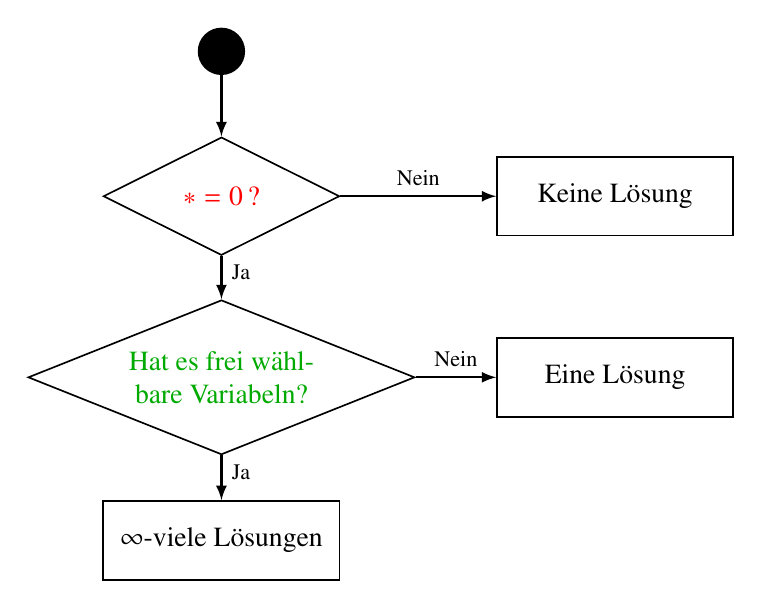
\begin{tikzpicture}[>=latex, scale=1,
    connection/.style={draw=black,thick},
	processStep/.style={rectangle,inner sep=3pt,minimum height=1cm,minimum width=3cm,draw=black,semithick},	
	decision/.style={diamond,inner sep=-1pt,minimum height=1.5cm,minimum width=3cm,draw=black,semithick,aspect=2.5},	
	start/.style={circle,inner sep=0pt,minimum size=16.5pt, draw=black,fill=black,semithick},	
   connection/.style={draw=black,thick,->},
]	

	\def\step{2.3};
	\def\shift{5};



	\node[start](begin) at(0,-0.2*\step){ };
	\node[decision](s0) at(0,-1*\step){\textcolor{red}{$\ast=0\,?$}};
	\node[decision,inner sep=1pt](s1) at(0,-2*\step){\textcolor{greenT}{\parbox{3cm}{\centering Hat es frei wähl-\\ bare Variabeln?}}};

	\node[processStep](s2) at(\shift,-1*\step){Keine Lösung};
	\node[processStep](s3) at(\shift,-2*\step){Eine Lösung};
	\node[processStep](s4) at(0,-2.9*\step){$\infty$-viele Lösungen};


	\draw[connection](begin)--(s0);
	\draw[connection](s0)--node[right,yshift=2pt]{\footnotesize Ja}(s1);
	\draw[connection](s0)--node[above]{\footnotesize Nein}(s2);
	\draw[connection](s1)--node[above]{\footnotesize Nein}(s3);
	\draw[connection](s1)--node[right,yshift=2pt]{\footnotesize Ja}(s4);

\end{tikzpicture}

\end{document}


\caption{Flussdiagramm für die Entscheidung, wieviele Lösungen ein
Gleichungssystem hat, basierend auf dem Schlusstableau
\label{lingl:flussdiagramm}}
\end{figure}

Nehmen wir an, dass auf der rechten Seite der Nullzeilen auch
nur Nullen stehen.
Offensichtlich können nur diejenigen Variablen bestimmt werden,
deren Spalten im Laufe des Verfahrens als Pivot-Spalten aufgetreten sind.
Alle anderen Variablen werden durch die vorhandenen Gleichungen nicht
bestimmt, und sind frei wählbar.

Der gesamte Enscheidungsprozess auf der Basis des
Schlusstableau~\eqref{rangdef} ist im Flussdiagramm
in Abbildung~\ref{lingl:flussdiagramm} zusammengefasst.

\begin{beispiel}
Man finde die Lösungsmenge des Gleichungssystems
\[
\begin{linsys}{4}
x&+&2y&+&3z&=&1\\
x&&&+&z&=&0\\
 &&2y&+&2z&=&1
\end{linsys}
\]
Der Gauss-Algorithmus liefert:
\begin{align*}
\begin{tabular}{|>{$}c<{$}>{$}c<{$}>{$}c<{$}|>{$}c<{$}|}
\hline
1%
\begin{picture}(0,0)
\color{red}\put(-3,4){\circle{12}}
\end{picture}%
&2&3&1\\
1&0&1&0\\
0%
\begin{picture}(0,0)
\color{blue}\drawline(-8,-2)(-8,24)(2,24)(2,-2)
\end{picture}%
&2&2&1\\
\hline
\end{tabular}
&\rightarrow
\begin{tabular}{|>{$}c<{$}>{$}c<{$}>{$}c<{$}|>{$}c<{$}|}
\hline
1&2&3&1\\
0&-2%
\begin{picture}(0,0)
\color{red}\put(-6,4){\circle{15}}
\end{picture}%
&-2&-1\\
0&2%
\begin{picture}(0,0)
\color{blue}\drawline(-8,-2)(-8,10)(2,10)(2,-2)
\end{picture}%
&2&1\\
\hline
\end{tabular}
\\
&\rightarrow
\begin{tabular}{|>{$}c<{$}>{$}c<{$}>{$}c<{$}|>{$}c<{$}|}
\hline
1&2%
\begin{picture}(0,0)
\color{blue}\drawline(-8,9)(-8,-2)(1,-2)(1,9)
\end{picture}%
&3&1\\
0&1&1&\frac12\\
0&0&0&\color{red}0\\
\hline
\end{tabular}
\rightarrow
\begin{tabular}{|>{$}c<{$}>{$}c<{$}:>{$}c<{$}|>{$}c<{$}|}
\hline
1&0&1&0\\
0&1&1&\frac12\\
\hdashline
0&0&0&\color{red}0\\
\hline
\end{tabular}
\end{align*}
Offenbar wird die letzte Gleichung gar nicht benötigt, die
Lösungsmenge kann aus den ersten zwei Gleichungen
abgelesen werden:
\[
\mathbb L=
\left\{
\left.
\begin{pmatrix}
0\\\frac12\\0
\end{pmatrix}
+x_3\begin{pmatrix}
-1\\-1\\1
\end{pmatrix}
\;
\right|\;
x_3\in\mathbb R
\right\}.
\]
\end{beispiel}

\subsection{Definition des Rangs}
\index{Rang}
Offenbar spielt die Zahl $r$, die Anzahl der Einsen im Schema (\ref{rangdef}),
eine wesentliche Rolle, wir nennen diese Zahl den Rang der Matrix.

\begin{definition}
Der Rang einer Matrix $A$ ist die maximale Anzahl linear unabhängiger Zeilen.
\end{definition}
\begin{satz}
Die maximale Anzahl linear unabhängiger Spalten einer Matrix $A$ ist
$\operatorname{Rang}A$.
\end{satz}
Aus dem Rang lässt sich also auch ermitteln, wie viele frei wählbare
Parameter in die Lösungsmenge eingehen.
\begin{satz}
Ist $A$ eine $m\times n$-Matrix mit $r=\operatorname{Rang}A$ 
und $b$ ein $m$-Vektor, dann gibt es $n-r$ Vektoren $\tilde a_1$
bis $\tilde a_{n-r}$ und einen Vektor $\tilde b$ so, dass
\[
\mathbb L
=
\{
\tilde b+x_1\tilde a_1+\dots+x_{n-r}\tilde a_{n+r}\;|\;x_1,\dots,x_{n-r}\in\mathbb R
\}
\]
die Lösungsmenge des Gleichungssystems $Ax=b$ ist.
\end{satz}

\subsection{Reduzierte Zeilenstufenform}
Das allgemeine Schlusstableau der Form (\ref{rangdef}) kann im Allgemeinen nur
erreicht werden, indem nach Bedarf Zeilen- und Spaltenvertauschungen vorgenommen
werden.
Während Zeilenvertauschungen unproblematisch sind, muss man bei
Spaltenvertauschungen sorgfältig darüber Buch führen, zu welcher Variablen
die Spalten gehören.
Dadurch wird der Algorithmus wesentlich komplizierter.
Gewünscht ist eine Variante des Algorithmus, die ohne Zeilenvertauschungen
auskommt, aber immer noch die gleich einfache Interpretation des
Schlusstableaus ermöglicht.

Wir überlegen uns zunächst, wie das Schlusstableau des modifizierten
Algorithmus aussehen müsste.
Das Tableau (\ref{rangdef}) enthält zwei Arten von Spalten:
Spalten mit einer $1$, welche dazu dienen die zugehörte Variable aus der
rechten Seite und eventuell frei wählbaren Variable zu berechnen, und
Spalten mit $*$, die frei wählbare Variablen anzeigen.
Spaltenvertauschungen auf dem Weg zu (\ref{rangdef}) verwenden immer nur Spalten
rechts von der aktuellen Pivot-Spalte, die Spalten links davon sind ja schon
ausgewertet worden.
Tauscht man die Spalten zurück, können zwar Spalten mit $*$ weiter links
landen, aber höchstens so, dass sich links davon eine $1$-Spalte finden
lässt, die die $1$ nicht weiter oben hat als der unterste $*$, das
Tableau sieht also ungefähr so aus:
\begin{center}
\begin{tabular}{| >{$}c<{$} >{$}c<{$} >{$}c<{$} >{$}c<{$} >{$}c<{$} >{$}c<{$} >{$}c<{$} >{$}c<{$} >{$}c<{$} >{$}c<{$} | >{$}c<{$}|}
\hline
1     &0     &*     &0     &0     &*     &0     &\dots &0     &*     &*\\
0     &1     &*     &0     &0     &*     &0     &\dots &0     &*     &*\\
0     &0     &0     &1     &0     &*     &0     &\dots &0     &*     &*\\
0     &0     &0     &0     &1     &*     &0     &\dots &0     &*     &*\\
0     &0     &0     &0     &0     &0     &1     &\dots &0     &*     &*\\
\vdots&\vdots&\vdots&\vdots&\vdots&\vdots&\vdots&\ddots&\vdots&\vdots&\vdots\\
0     &0     &0     &0     &0     &0     &0     &\dots &1     &*     &*\\
\hdashline
0     &0     &0     &0     &0     &0     &0     &\dots &0     &0     &\color{red}*\\
\vdots&\vdots&\vdots&\vdots&\vdots&\vdots&\vdots&\ddots&\vdots&\vdots&\color{red}\vdots\\
0     &0     &0     &0     &0     &0     &0     &\dots &0     &0     &\color{red}*\\
\hline
\end{tabular}
\end{center}
Auch in dieser Form lassen sich die Fragen bezüglich der Anzahl der Lösung
direkt aus dem Tableau ablesen.
Ist einer der roten $\color{red}*$ von Null verschieden, gibt es keine Lösung,
andernfalls gibt es unendlich viele Lösungen, wenn frei wählbare Variablen
in Spalten mit $*$ vorhanden sind.
Die Lösungsmenge lässt sich wieder ablesen, indem man die frei wählbaren
Variablen auf die rechte Seite bringt.

Nachdem nun klar ist, wie ein Schlusstableau ohne Spaltenvertauschungen aussehen
wird, müssen wir den Algorithmus so formulieren, dass wir das Tableau direkt
finden können, ohne Umweg über Vertauschungen und Rückvertauschungen.
Im bisherigen Algorithmus wird eine Spaltenvertauschung unumgänglich, wenn
im nächsten Pivot-Feld und in allen Feldern der Spalte unterhalb des Pivot-Feldes
nur $0$ stehen:
\begin{center}
\begin{tabular}{| >{$}c<{$} >{$}c<{$} >{$}c<{$} >{$}c<{$} >{$}c<{$} | >{$}c<{$} |}
\hline
\qquad\qquad &*     &*     &*     &\qquad\qquad&*     \\
       &\vdots&\vdots&\vdots&      &\vdots\\
       &1     &*     &*     &      &*     \\
       &0     &0\begin{picture}(0,0)
\color{red}\put(-3.5,3){\circle{15}}
\end{picture}&*     &      &*     \\
       &\vdots&\vdots&\vdots&      &\vdots\\
       &0     &0     &*     &      &*     \\
\hline
\end{tabular}
\end{center}
Die zur Pivot-Spalte gehörige Variable kann auf keinen Fall bestimmt werden,
denn dazu wäre ja ein von Null verschiedenes Element an der Pivot-Position
oder darunter notwendig.
Es steht also jetzt schon fest, dass diese Variable frei wählbar ist.
Man kann daher diese Spalte überspringen, und in der nächsten Spalte nach
einem geeigneten Pivot-Element suchen:
\begin{align*}
\begin{tabular}{| >{$}c<{$} >{$}c<{$} >{$}c<{$} >{$}c<{$} >{$}c<{$} | >{$}c<{$} |}
\hline
\qquad\qquad &*     &*     &*     &\qquad\qquad&*     \\
       &\vdots&\vdots&\vdots&      &\vdots\\
       &1     &*     &*     &      &*     \\
       &0     &0     &*
\begin{picture}(0,0)
\color{red}\put(-3.5,3){\circle{15}}
\end{picture}
                            &      &*     \\
       &\vdots&\vdots&\vdots&      &\vdots\\
       &0     &0     &*     &      &*     \\
\hline
\end{tabular}
&\rightarrow
\begin{tabular}{| >{$}c<{$} >{$}c<{$} >{$}c<{$} >{$}c<{$} >{$}c<{$} | >{$}c<{$} |}
\hline
\qquad\qquad&*     &*     &*     &\qquad\qquad&*     \\
            &\vdots&\vdots&\vdots&            &\vdots\\
            &1     &*     &*     &            &*     \\
            &0     &0     &1     &            &*     \\
            &\vdots&\vdots&\vdots&            &\vdots\\
            &0     &0     &0     &            &*     \\
\hline
\end{tabular}
\end{align*}
Die Einsen entstehen jetzt nicht mehr entlang der Diagonalen, sondern
entlang einer Treppe, in der einzelne Stufen auch etwas breiter sein können.
Das Rückwärtseinsetzen funktioniert weiterhin, wobei natürlich nur
Spalten bearbeitet werden können, in denen sich eine Pivot-Position
befindet.

\begin{beispiel}
Man finde die Lösungsmenge des Gleichungssystems
\[
\begin{linsys}{5}
3x&+&6y& &  &+&12v&=& 6\phantom{.}\\
 x&+&2y&+&3z&+&25v&=&17\phantom{.}\\
2x&+&4y&+&3z&+&29v&=&19.
\end{linsys}
\]
In Tableauform vollzieht sich der modifizierte Gauss-Algorithmus jetzt wie
folgt:
\begin{align*}
\begin{tabular}{| >{$}c<{$} >{$}c<{$} >{$}c<{$} >{$}c<{$} | >{$}c<{$} |}
\hline
  3
\begin{picture}(0,0)
\color{red}\put(-3.5,3){\circle{12}}
\end{picture}
   &  6&  0& 12&  6\\
  1&  2&  3& 25& 17\\
  2&  4&  3& 29& 19\\
\hline
\end{tabular}
&\rightarrow
\begin{tabular}{| >{$}c<{$} >{$}c<{$} >{$}c<{$} >{$}c<{$} | >{$}c<{$} |}
\hline
  1&  2&  0&  4&  2\\
  0&  0&  3
\begin{picture}(0,0)
\color{red}\put(-3.5,3){\circle{12}}
\end{picture}
           & 21& 15\\
  0&  0&  3& 21& 15\\
\hline
\end{tabular}
\rightarrow
\begin{tabular}{| >{$}c<{$} >{$}c<{$} >{$}c<{$} >{$}c<{$} | >{$}c<{$} |}
\hline
  1&  2&  0&  4&  2\\
  0&  0&  1&  7&  5\\
  0&  0&  0&  0&  0\\
\hline
\end{tabular}
\end{align*}
Per Zufall ist das Element oberhalb der $1$ in der dritten Spalte auch schon $0$,
es gibt also für das Rückwärtseinsetzen nichts mehr zu tun.

Man kann jetzt die Lösungsmenge ablesen: frei wählbar sind die Variablen 
$y$ und $z$, die Variablen $x$ und $v$ können durch $y$ und $v$ ausgedrückt
werden
\begin{align*}
x&=2-2y-4v\\
z&=5-7v.
\end{align*}
Die Lösungsmenge ist daher
\[
{\mathbb L}
=
\left\{
\left.
\begin{pmatrix}x\\y\\z\\v\end{pmatrix}
=
\begin{pmatrix}2\\0\\5\\0\end{pmatrix}
+y\begin{pmatrix}-2\\1\\0\\0\end{pmatrix}
+v\begin{pmatrix}-4\\0\\-7\\1\end{pmatrix}\;\right|
y,v\in\mathbb R
\right\}.
\]
\end{beispiel}

Das nach diesem modifizierten Algorithmus gefundene Schlusstableau heisst
die {\em reduzierte Zeilenstufenform}, englisch auch {\em reduced row echelon form}.
\index{Zeilenstufenform, reduzierte}
\index{rref}
\index{reduced row echelon form}
Leistungsfähige Taschenrechner und Programme zur Matrizenrechnung stellen
eine üblicherweise \texttt{rref} genannte Funktion zur Verfügung, welche die 
Zeilenstufenform einer beliebigen Matrix berechnen kann.


%
% simultan.tex -- mehrere Gleichungssysteme gleichzeitig lösen
%
% (c) 2009 Prof Dr Andreas Mueller, Hochschule Rapperswil
%
\section{Mehrere rechte Seiten\label{section:mehrere rechte seiten}}
\rhead{Simultane Lösung mit mehreren rechten Seiten}
Bis jetzt wurde der Gauss-Algorithmus immer nur auf Gleichungen mit
einer konstanten rechten Seite angewendet.
Der Gauss-Algorithmus kann noch wesentlich mehr.
Er kann in einem Durchgang ein Gleichungssysteme für mehrere verschiedene
rechte Seiten lösen, die wird in Abschnitt~\ref{simultan} gezeigt.
Er kann aber auch Gleichungssysteme lösen, in denen die rechte
Seite eine Linearform ist (Abschnitt~\ref{subsection:rechte seite linear}).

%
% Mehrere Gleichungssysteme simultan lösen
%
\subsection{Mehrere Gleichungssysteme simultan lösen\label{simultan}}
Mit dem Gauss-Algorithmus kann man gleichzeitig mehrere Gleichungssysteme
lösen, die sich nur in den rechten Seiten unterscheiden.
Die rechten Seiten haben nämlich auf den Gang der Rechnung keinen
Einfluss.
So kann man die beiden Gleichungssysteme
\begin{align*}
\frac12x+\frac{\sqrt{3}}2y&=1
&
\frac12x+\frac{\sqrt{3}}2y&=0
\\
-\frac{\sqrt{3}}2x+\frac12y&=0
&
-\frac{\sqrt{3}}2x+\frac12y&=1
\end{align*}
in einem Durchgang lösen:
\begin{align*}
\begin{tabular}{|>{$}c<{$}>{$}c<{$}|>{$}c<{$}>{$}c<{$}|}
\hline
\frac12%
\begin{picture}(0,0)
\color{red}\put(-3.5,3){\circle{15}}
\end{picture}%
&\frac{\sqrt{3}}2&1&0\\
-\frac{\sqrt{3}}2&\frac12&0&1\\
\hline
\end{tabular}
&\rightarrow
\begin{tabular}{|>{$}c<{$}>{$}c<{$}|>{$}c<{$}>{$}c<{$}|}
\hline
1&\sqrt{3}&2&0\\
-\frac{\sqrt{3}}2%
\begin{picture}(0,0)
\color{blue}\drawline(-22,-4)(-22,13)(1,13)(1,-4)
\end{picture}%
&\frac12&0&1\\
\hline
\end{tabular}
\rightarrow
\begin{tabular}{|>{$}c<{$}>{$}c<{$}|>{$}c<{$}>{$}c<{$}|}
\hline
1&\sqrt{3}&2&0\\
0&2%
\begin{picture}(0,0)
\color{red}\put(-3,4){\circle{12}}
\end{picture}%
&\sqrt{3}&1\\
\hline
\end{tabular}
\\
&\rightarrow
\begin{tabular}{|>{$}c<{$}>{$}c<{$}|>{$}c<{$}>{$}c<{$}|}
\hline
1&\sqrt{3}%
\begin{picture}(0,0)
\color{blue}\drawline(-16,11)(-16,-3)(1,-3)(1,11)
\end{picture}%
&2&0\\
0&1&\frac{\sqrt{3}}2&\frac12\\
\hline
\end{tabular}
\rightarrow
\begin{tabular}{|>{$}c<{$}>{$}c<{$}|>{$}c<{$}>{$}c<{$}|}
\hline
1&0&\frac12&-\frac{\sqrt{3}}2\\
0&1&\frac{\sqrt{3}}2&\frac12\\
\hline
\end{tabular}
\end{align*}
Das erste Gleichungssystem hat also die Lösung
$(x,y)=(\frac12,\frac{\sqrt{3}}2)$,
das zweite
$(x,y)=(-\frac{\sqrt{3}}2, \frac12)$.

Die spezielle Wahl der rechten Seiten erlaubt auch, aus den
beiden gefundenen Lösungen die Lösung für jede beliebige rechte
Seite zusammenzusetzen. Wenn nämlich auf der rechten
Seite die Zahlen $b_1$ und $b_2$ stehen sollen, dann
bedeutet dies offenbar, dass wir $b_1$ mal die erste Lösung
und $b_2$ mal die zweite Lösung zusammennehmen müssen, um
die verlangten rechten Seiten zu finden.
Also
\[
x=\frac12b_1-\frac{\sqrt{3}}2b_2,\qquad y=\frac{\sqrt{3}}2b_1+\frac12b_2.
\]
Durch Einsetzen in die ursprüngliche Gleichung kann man die
Lösung überprüfen.

%
% Linearform als rechte Seite
%
\subsection{Linearform als rechte Seite\label{subsection:rechte seite linear}}
Das Gauss-Tableau ist nur eine abgekürzte Schreibweise für ein Gleichungssystem.
In Abschnitt~\ref{subsection:sonderfaelle} haben wir die Spalten mit
den Variablennamen beschriftete, so dass wir sogar die Variablennamen
aus dem Tableau wieder bekommen können.
Die Übersetzungsregel können wir schematisch als
\[
\begin{tabular}{|>{$}c<{$} >{$}c<{$} >{$}c<{$} >{$}c<{$}|}
\hline
x_1&x_2&\dots&x_n\\
\hline
a_{11}&a_{12}&\dots&a_{1n}\\
\vdots&\vdots&\ddots&\vdots\\
a_{m1}&a_{m2}&\dots&a_{mn}\\
\hline
\end{tabular}
\quad
\leftrightarrow
\quad
\begin{linsys}{3}
a_{11}x_1&+&a_{12}x_2&+&\dots &+&a_{1n}x_n\\
\vdots\hspace*{1em} & &\vdots\hspace*{1em} & &\ddots& &\vdots\hspace*{1em}\\
a_{m1}x_1&+&a_{m2}x_2&+&\dots &+&a_{mn}x_n\\
\end{linsys}
\]
darstellen.
Damit lässt sich aber auch ein Gleichungssystem in ein Tableau übersetzen,
welches Linearformen auf der rechten Seite hat.
Das Gleichheitszeichen wird zum Vertikalstrich wie früher, und die
Linearformen auf der rechten Seite werden zu Spalten, die mit den
Variablen der Linearformen beschriftet sind.

\begin{beispiel}
Als Beispiel übersetzen wir
\begin{equation}
\begin{linsys}{4}
3x_1&+&4x_2&=& 9y_1&+4y_2\\
5x_1&+&7x_2&=&20y_1&+9y_2
\end{linsys}
\quad\leftrightarrow\quad
\begin{tabular}{| >{$}c<{$} >{$}c<{$}| >{$}c<{$} >{$}c<{$}|}
\hline
x_1&x_2&y_1&y_3\\
\hline
3&4&9&4\\
5&7&20&9\\
\hline
\end{tabular}
\label{skript:rechtslinearubers}
\end{equation}

Die Lösung des Gleichungssystems~\eqref{skript:rechtslinearubers} 
funktioniert mit dem Gaussalgorithmus wie bisher.
Wir führen den Gauss-Algorithmus durch:
\begin{align*}
\begin{tabular}{| >{$}c<{$} >{$}c<{$}| >{$}c<{$} >{$}c<{$}|}
\hline
x_1&x_2&y_1&y_3\\
\hline
3&4&9&4\\
5&7&20&9\\
\hline
\end{tabular}
&\rightarrow
\begin{tabular}{| >{$}c<{$} >{$}c<{$}| >{$}c<{$} >{$}c<{$}|}
\hline
x_1&x_2&y_1&y_3\\
\hline
1&\frac{4}{3}&3&\frac{4}{3}\\
0&\frac{1}{3}&5&\frac{7}{3}\\
\hline
\end{tabular}
\rightarrow
\begin{tabular}{| >{$}c<{$} >{$}c<{$}| >{$}c<{$} >{$}c<{$}|}
\hline
x_1&x_2&y_1&y_3\\
\hline
1&0&-17&-8\\
0&1& 15& 7\\
\hline
\end{tabular}
\end{align*}
Die Rückübersetzung davon ergibt
\[
\begin{linsys}{3}
x_1& &   &=&-17y_1&-&8y_2\\
   & &x_2&=& 15y_1&+&7y_2
\end{linsys}
\]
Setzen wir diese Linearformen für $x_1$ und $x_2$ in die ursprünglichen
Gleichungen~\eqref{skript:rechtslinearubers} ein, erhalten
wir
\begin{align*}
3x_1+4x_2
&=
3(-17y_1-8y_2)+4(15y_1+7y_2)
=
-51y_1-24y_2+60y_1+28y_2
=
9y_1+4y_2
\\
5x_1+7x_1
&=
5(-17y_1-8y_2)+7(15y_1+7y_2)
=
-85y_1-40y_2+105y_1+49y_2
=
20y_1+9y_2,
\end{align*}
also genau die ursprünglichen Gleichungen.
Der Gauss-Algorithmus hat also tatsächlich die Lösungen des
Gleichungssystems~\eqref{skript:rechtslinearubers} als
Linearformen in den Variablen $y_1$ und $y_2$ der rechten Seite
geliefert.
\end{beispiel}

Dies gilt natürlich ganz allgemein.
Auf der rechten Seite des Tableaus finden während des Gauss-Algorithmus
nur Multiplikationen mit Zahlen und Additionen statt.
Diese Operationen kann man getrennt für jeden einzelnen Term der
Form $b_{ij}y_j$ auf der rechten Seite durchführen.
In diesem Lichte sind die Spalten auf der rechten Seite des Tableaus
nur ein ``Buchhaltungshilfsmittel'', mit dem wir sicherstellen, dass
die Variablen auf der rechten Seite nicht durcheinander geraten.

Es gibt keinen Grund, warum die Anzahl der Variablen auf der rechten
Seite genau $n$ sein soll.
Ganz allgemein können wir ein Gleichungssystem mit $m$ Gleichungen
und $n$ unbekannten sowie $l$ Variablen auf der  rechten Seite
in ein Tableau mit $m$ Zeilen und $n$ Spalten links und $l$
Spalten rechts vom Vertikalstrich übersetzen:
\[
\begin{linsys}{5}
a_{11}x_1&+&\dots&+&a_{1n}x_n&=&b_{11}y_1&+&\dots&+&b_{1l}y_l\\
\vdots*\hspace{1em}&&\ddots&&\vdots\hspace*{1em}&&\vdots\hspace*{1em}&&\ddots&&\vdots\hspace*{1em}\\
a_{m1}x_1&+&\dots&+&a_{mn}x_n&=&b_{m1}y_1&+&\dots&+&b_{ml}y_l\\
\end{linsys}
\quad\rightarrow\quad
\begin{tabular}{| >{$}c<{$}>{$}c<{$}>{$}c<{$}|>{$}c<{$}>{$}c<{$}>{$}c<{$}|}
\hline
x_1&\dots&x_n&y_1&\dots&y_l\\
\hline
a_{11}&\dots&a_{1n}&b_{11}&\dots&b_{1l}\\
\vdots&\ddots&\vdots&\vdots&\ddots&\vdots\\
a_{m1}&\dots&a_{mn}&b_{m1}&\dots&b_{ml}\\
\hline
\end{tabular}
\]
Das Schlusstableau nach Anwendung des Gauss-Algorithmus ist dann
\begin{equation}
\begin{tabular}{|>{$}c<{$}>{$}c<{$}>{$}c<{$}:>{$}c<{$}>{$}c<{$}>{$}c<{$}|
>{$}c<{$}>{$}c<{$}>{$}c<{$}|}
\hline
x_{i_1}&\dots&x_{i_r}
	&x_{i_{r+1}}&\dots&x_{i_n}
		&y_1&\dots&y_l\\
\hline
1&\dots &0     
	&\color{green}c_{1,r+1}&\color{green}\dots &\color{green}c_{1n}
		&d_{11}&\dots&d_{1l}\\
\vdots&\ddots&\vdots
	&\color{green}\vdots&\color{green}\ddots&\color{green}\vdots
		&\vdots&\ddots&\vdots\\
0&\dots &1
	&\color{green}c_{r,r+1}&\color{green}\dots &\color{green}c_{rn}
		&d_{r1}&\dots&d_{rl}\\
\hdashline
0&\dots &0     
	&0&\dots &0
		&\color{red}d_{r+1,1}&\color{red}\dots&\color{red}d_{r+1,l}\\
\vdots&\ddots&\vdots
	&\vdots&\ddots&\vdots
		&\color{red}\vdots&\color{red}\ddots&\color{red}\vdots\\
0&\dots &0
	&0&\dots &0
		&\color{red}d_{m1}&\color{red}\dots&\color{red}d_{ml}\\
\hline
\end{tabular}
\label{skript:simultan:schluss}
\end{equation}
Dabei ist zu beachten, dass Infolge möglicher Spaltenvertauschungen
die Variablen $x_i$ nicht mehr ihre ursprünglichen Plätze haben,
sondern, dies wird durch die neuen Indizes $i_1,\dots,i_n$
ausgedrückt.

Die {\color{red}roten} Koeffizienten bestimmen, ob das Gleichungssystem
überhaupt eine Lösung hat.
Wenn eine der Linearformen gebildet aus den {\color{red}roten} Koeffizienten
einen Wert $\mathstrut \ne 0$ liefert für die gegebenen Werte der
$y$-Variablen, dann ist das Gleichungssystem nicht lösbar.
Wenn man also wissen will, für welche Werte von $y_i$ das Gleichungssystem
überhaupt lösbar ist, muss man das kleiner Gleichungssystem
\[
\begin{linsys}{3}
{\color{red}d_{r+1,1}}y_1&+&\dots&+&{\color{red}d_{r+1,l}}y_l&=&0\\
\vdots\hspace*{1em}&&\ddots&&\vdots\hspace*{1em}&&\vdots\hspace*{0.7mm}\\
{\color{red}d_{m1}}y_1&+&\dots&+&{\color{red}d_{ml}}y_l&=&0\\
\end{linsys}
\]
lösen, was natürlich wiederum mit dem Gauss-Algorithmus geschehen kann.
Insbesondere ist es für $l>m-r$ immer möglich, eine Kombination von $y_i$
zu finden, für die der {\color{red}rote} Teil des Gleichungssystems
verschwindet.

Wenn der {\color{red}rote} Teil verschwindet, hat das Gleichungssystem
mindestens eine Lösung.
Wenn $n>r$ ist, dann sind die {\color{green}grünen} Variablen $x_{i_{r+1}}$
bis $x_{i_n}$ frei wählbar, es gibt also unendlich viele Lösungen.
die ersten $r$ Variablen $x_{i_1}$ bis $x_{i_r}$ sind dann durch die
{\color{green}frei wählbaren} Variablen eindeutig bestimmt.
Aus dem Tableau~\eqref{skript:simultan:schluss} kann man die Gleichungen
\[
\begin{linsys}{6}
x_{i_1}&=&d_{11}y_1&+&\dots&+&d_{1l}y_l&-&{\color{green}c_{1,r+1}}x_{i_{r+1}}&-&\dots&-&{\color{green}c_{1n}}x_{i_n}\\
\vdots\hspace*{0.5em} && \vdots\hspace*{1em} && \ddots && \vdots\hspace*{1em} && \vdots\hspace*{1em} && \ddots && \vdots\hspace*{1em}\\
x_{i_r}&=&d_{r1}y_1&+&\dots&+&d_{rl}y_l&-&{\color{green}c_{r,r+1}}x_{i_{r+1}}&-&\dots&-&{\color{green}c_{rn}}x_{i_n}\\
\end{linsys}
\]
für die Variablen $x_{i_1}$ bis $x_{i_r}$ ablesen.
Dies lässt sich natürlich auch in der Form einer Lösungsmenge schreiben.

%
% Standardbasisvektoren
%
\subsection{Standardbasisvektoren als rechte Seiten%
\label{skript:subsection:standardrs}}
Ein interessanter Spezialfall liegt vor, wenn man ein Gleichungssystem
für die rechten Seiten 
\[
e_1=\begin{pmatrix}1\\0\\0\end{pmatrix},\qquad
e_2=\begin{pmatrix}0\\1\\0\end{pmatrix},\qquad
e_3=\begin{pmatrix}0\\0\\1\end{pmatrix}
\]
bereits gelöst und die Lösungsvektoren
\[
c_1=\begin{pmatrix} c_{11}\\ c_{21}\\ c_{31} \end{pmatrix},\qquad
c_2=\begin{pmatrix} c_{12}\\ c_{22}\\ c_{32} \end{pmatrix},\qquad
c_3=\begin{pmatrix} c_{13}\\ c_{23}\\ c_{33} \end{pmatrix}
\]
gefunden hat.
Da die allgemeine rechte Seite
\[
b=\begin{pmatrix}
b_1\\b_2\\b_3
\end{pmatrix}
=
b_1 \begin{pmatrix}1\\0\\0\end{pmatrix}
+
b_2 \begin{pmatrix}0\\1\\0\end{pmatrix}
+
b_3 \begin{pmatrix}0\\0\\1\end{pmatrix}
=
b_1 e_1 + b_2 e_2 + b_3 e_3
\]
als Linearkombination der Standardbasisvektoren $e_i$ geschrieben
werden kann, kann man die Lösung des Gleichungssystems mit rechter
Seite $b$ auch als ein Beispiel für ein Gleichungssystem mit rechten
Seiten betrachten, die Linearformen in den `Variablen' $b_i$ sind.
Das Tableau dazu ist
\[
\begin{tabular}{|>{$}c<{$}>{$}c<{$}>{$}c<{$}|>{$}c<{$}|}
\hline
x_1&x_2&x_3&\\
\hline
a_{11}&a_{12}&a_{13}&b_1\\
a_{21}&a_{22}&a_{23}&b_2\\
a_{31}&a_{32}&a_{33}&b_3\\
\hline
\end{tabular}
\quad\rightarrow\quad
\begin{tabular}{|>{$}c<{$}>{$}c<{$}>{$}c<{$}|>{$}c<{$}>{$}c<{$}>{$}c<{$}|}
\hline
x_1&x_2&x_3&b_1&b_2&b_3\\
\hline
a_{11}&a_{12}&a_{13}&1&0&0\\
a_{21}&a_{22}&a_{23}&0&1&0\\
a_{31}&a_{32}&a_{33}&0&0&1\\
\hline
\end{tabular}
\]
Wendet man darauf den Gauss-Algorithmus an, bekommt man das
Tableau
\[
\begin{tabular}{|>{$}c<{$}>{$}c<{$}>{$}c<{$}|>{$}c<{$}>{$}c<{$}>{$}c<{$}|}
\hline
x_1&x_2&x_3&b_1&b_2&b_3\\
\hline
1&0&0&c_{11}&c_{12}&c_{13}\\
0&1&0&c_{21}&c_{22}&c_{23}\\
0&0&1&c_{31}&c_{32}&c_{33}\\
\hline
\end{tabular},
\]
welches mit den Gleichungen
\[
\begin{linsys}{3}
x_1&=&c_{11}b_1&+&c_{12}b_2&+&c_{13}b_3\\
x_2&=&c_{21}b_1&+&c_{22}b_2&+&c_{23}b_3\\
x_3&=&c_{31}b_1&+&c_{32}b_2&+&c_{33}b_3\\
\end{linsys}
\]
gleichbedeutend ist.
Diese kann man auch vektoriell als
\[
x = b_1 c_1 + b_2 c_2 + b_3 c_3
\]
schreiben.

Man kann also ein allgemeines Lösungsverfahren für lineare Gleichungssysteme
mit wie folgt konzipieren.
Zunächst bildet man das Gauss-Tableau
\begin{center}
\begin{tabular}{|>{$}c<{$}>{$}c<{$}>{$}c<{$}|>{$}c<{$}>{$}c<{$}>{$}c<{$}|}
\hline
a_{11}&a_{12}&a_{13}&1&0&0\\
a_{21}&a_{22}&a_{23}&0&1&0\\
a_{31}&a_{32}&a_{33}&0&0&1\\
\hline
\end{tabular}
\end{center}
welches man anschliessend mit dem Gauss-Algorithmus in das Tableau
\begin{center}
\begin{tabular}{|>{$}c<{$}>{$}c<{$}>{$}c<{$}|>{$}c<{$}>{$}c<{$}>{$}c<{$}|}
\hline
1&0&0&c_{11}&c_{12}&c_{13}\\
0&1&0&c_{21}&c_{22}&c_{23}\\
0&0&1&c_{31}&c_{32}&c_{33}\\
\hline
\end{tabular}
\end{center}
umwandelt.
Dann baut man die Lösung aus den Zahlen $c_{ij}$ und der rechten
Seite $b$ zusammen.
Die Berechnung der $c_{ij}$ muss nur einmal
erfolgen, danach kann die Lösung mit verschiedenen rechten Seiten
$b$ bestimmt werden.


%
% matrizen.tex -- Matrizen und Vektoren
%
% (c) 2009 Prof Dr Andreas Mueller, Hochschule Rapperswil
%
\section{Notation: Matrizen und Vektoren}
\rhead{Notation: Matrizen und Vektoren}
Viele der Operationen im Lösungsverfahren für lineare Gleichungssysteme,
sind unabhängig von ihrem Bezug zu einem Gleichungssystem sinnvoll.
In der Tableaudarstellung haben wir auch eine Notation verwendet,
in der die Unbekannten überhaupt nicht mehr vorkommen.
Dies kann jedoch nicht nur eine praktische Abkürzung sein, es muss mehr
dahinter stecken.
In diesem Abschnitt definieren wir die Vektoren und Matrizen, die zu
einem Gleichungssystem gehören.

\subsection{Vektoren}
\subsubsection{Definition von Zeilen- und Spaltenvektoren}
Die Operationen im Lösungsverfahren erfolgten jeweils Zeilen- oder Spaltenweise,
es ist daher sinnvoll, die Zeilen oder Spalten als eigene vollwertige 
mathematische Objekte zu definieren.

\begin{definition}
Das Zahlenschema
\[
\begin{pmatrix}
a_1&a_2&\dots&a_n
\end{pmatrix}
\]
mit $a_i\in\mathbb R$ heisst ein $n$-dimensionaler Zeilenvektor.
Das Zahlenschema
\[
\begin{pmatrix}
b_1\\b_2\\\vdots\\b_m
\end{pmatrix}
\]
heisst $m$-dimensionaler Spaltenvektor.
\end{definition}
Die Linearformen entsprechen also Zeilenvektoren, die rechte
Seite des Gleichungssystems ist ein Spaltenvektor.

Zeilen oder Spaltenvektoren kürzen wir ab als ein einzelnes
Zeichen, zum Beispiel
\[
a
=
\begin{pmatrix}
a_1&a_2&\dots&a_n
\end{pmatrix},\qquad
b=\begin{pmatrix}
1\\2\\3
\end{pmatrix}.
\]

\subsubsection{Rechenoperationen mit Vektoren}
Für Zeilen- oder Spaltenvektoren können wir die Addition von
Vektoren und die Multiplikation mit reellen Zahlen definieren.
Damit das überhaupt gehen kann, müssen die Vektoren natürlich
die gleiche Länge (Dimension) haben.
Die Operationen erfolgen elementweise:

\begin{definition}
Seien $a$ und $a'$ zwei $n$-dimensionale Zeilenvektoren,
\begin{align*}
a&=\begin{pmatrix}a_1&a_2&\dots&a_n\end{pmatrix}
\\
a'&=\begin{pmatrix}a'_1&a'_2&\dots&a'_n\end{pmatrix}
\end{align*}
und $\lambda\in\mathbb R$, dann sind die Summe $a+a'$ und das
Produkt $\lambda a$ wie folgt definiert:
\begin{align*}
a+a'&=\begin{pmatrix}a_1+a'_1&a_2+a'_2&\dots&a_n+a'_n\end{pmatrix}
\\
\lambda a&=\begin{pmatrix}\lambda a_1&\lambda a_2&\dots&\lambda a_n\end{pmatrix}
\end{align*}
Sind $b$ und $b'$ zwei $m$-dimensionale Spaltenvektoren
\begin{align*}
b&=\begin{pmatrix}b_1\\b_2\\\vdots\\b_m\end{pmatrix},
&
b'&=\begin{pmatrix}b'_1\\b'_2\\\vdots\\b'_m\end{pmatrix}
\end{align*}
dann, sind die Summe $b+b'$ und das Produkt $\lambda b$ wie folgt 
definiert:
\begin{align*}
b+b'&=\begin{pmatrix}
b_1+b'_1\\
b_2+b'_2\\
\vdots\\
b_m+b'_m\\
\end{pmatrix},
&
\lambda b&=\begin{pmatrix}
\lambda b'_1\\
\lambda b'_2\\
\vdots\\
\lambda b'_m
\end{pmatrix}
\end{align*}
\end{definition}
Die Operationen {\bf E} und {\bf I} können wir jetzt mit Vektoren
beschreiben.
Die Zeile mit der Nummer $i$ ist offenbar ein
$n+1$-dimensionaler Zeilenvektoren $z_i$
\[
z_i=\begin{pmatrix}a_{i1}&a_{i2}&\dots&a_{im}&b_i\end{pmatrix}.
\]
Die Operation {\bf I} für die $i$-te Zeile bedeutet jetzt, dass man
den Zeilenvektor $z_i$ ersetzt durch den neuen Zeilenvektor
\[
\frac1{a_{ii}}z_i
=
\frac1{a_{ii}}
\begin{pmatrix}a_{i1}&a_{i2}&\dots&a_{im}&b_i\end{pmatrix}
=
\begin{pmatrix}\frac{a_{i1}}{a_{ii}}&\frac{a_{i2}}{a_{ii}}&\dots&\frac{a_{im}}{a_{ii}}&\frac{b_i}{a_{ii}}\end{pmatrix}
\]
Bei der Operation {\bf E} wird der Zeilenvektor $z_j$
verringert um das $a_{ji}$-fache des Zeilenvektors $z_i$, also
\[
z_j \leftarrow z_j-a_{ji}z_i.
\]

\subsubsection{Gleichungssystem in Vektorschreibweise}
Auch das Gleichungssystem selbst können wir mit Hilfe von Spaltenvektoren
schreiben.
Betrachten wir die Spalten mit der Nummer $k$ als Spaltenvektor $a_k$,
also
\[
a_k=\begin{pmatrix}a_{1k}\\a_{2k}\\\dots\\a_{mk}\end{pmatrix},
\]
und die rechten Seiten des Gleichungssystems wie früher als Spaltenvektor $b$,
dann können wir das Gleichungssystem schreiben als
\[
x_1\begin{pmatrix}a_{11}\\a_{21}\\\vdots\\a_{m1}\end{pmatrix}
+
x_2\begin{pmatrix}a_{12}\\a_{22}\\\vdots\\a_{m2}\end{pmatrix}
+
\dots
+
x_n\begin{pmatrix}a_{1n}\\a_{2n}\\\vdots\\a_{mn}\end{pmatrix}
=
\begin{pmatrix}b_1\\b_2\\\vdots\\b_m\end{pmatrix}
\]
oder kurz
\[
a_1x_1+a_2x_2+\dots+a_nx_n=b.
\]

\subsubsection{Spezielle Vektoren\label{speziellevektoren}}
Die folgenden speziellen Vektoren sind oft nützlich.
Der Nullvektor besteht
aus lauter Nullen, wir schreiben dafür
\[
0=\begin{pmatrix}0\\\vdots\\0\end{pmatrix}.
\]
Im Verfahren für die simultane Lösung von Gleichungssystemen haben
wir spezielle rechte Seiten verwendet, welche bis auf eine Stelle aus lauter
Nullen bestehen.
Diese Vektoren bezeichnen wir in Zukunft mit
\[
e_1=\begin{pmatrix}1\\0\\\vdots\\0\end{pmatrix},
\qquad
e_2=\begin{pmatrix}0\\1\\\vdots\\0\end{pmatrix},
\qquad
e_n=\begin{pmatrix}0\\0\\\vdots\\1\end{pmatrix}.
\]

\subsection{Matrizen\label{skript:subsection:matrizen}}
\subsubsection{Definition einer Matrix}
Die Formulierung mit Zeilen- und Spaltenvektoren ist immer noch etwas umständlich,
wir würden erwarten, dass auch das ganze Koeffizientenschema $(a_{ij})$
eine eigenständiges mathematisches Objekt ist, immerhin bestimmt es den
Gang des Lösungsverfahrens vollständig.

\begin{definition}
Das rechteckige Zahlenschema
\[
A=
\begin{pmatrix}
a_{11}&a_{12}&\dots&a_{1n}\\
a_{21}&a_{22}&\dots&a_{2n}\\
\vdots&\vdots&\ddots&\vdots\\
a_{m1}&a_{m2}&\dots&a_{mn}\\
\end{pmatrix}
\]
heisst $m\times n$-Matrix.
\end{definition}

\subsubsection{Produkt einer Matrix mit einem Vektor}
\index{Produkt!Matrix mal Vektor}
\index{Matrizenprodukt}
Um das Gleichungssystem mit der Koeffizientenmatrix $A$ zu beschreiben
fehlt uns jetzt noch eine Verknüpfung zwischen Matrizen und
Vektoren.
Die folgende Definition tut, was wir uns wünschen.
\begin{definition}
Ist $A$ eine $m\times n$-Matrix und $x$ ein $n$-dimensionaler Spaltenvektor,
dann definieren wir das Produkt $Ax$ also den $m$-dimensionalen
Spaltenvektor
\[
\begin{pmatrix}
a_{11}x_1+a_{12}x_2+\dots+a_{1n}x_n\\
a_{21}x_1+a_{22}x_2+\dots+a_{2n}x_n\\
\vdots\\
a_{m1}x_1+a_{m2}x_2+\dots+a_{mn}x_n\\
\end{pmatrix}
\]
Das Element $b_i$ in der $i$-ten Zeile dieses Spaltenvektors ist
\[
b_i=\sum_{j=1}^na_{ij}x_j.
\]
\end{definition}
Die Multiplikation $Ax$ erfolgt also, indem die Zeilen von $A$
elementweise mit der Spalte $x$ multipliziert, und dann alle Produkte
aufaddiert werden (``Zeile $\strut \times\mathstrut$ Spalte'').

\begin{beispiel} Sei
\[
A=\begin{pmatrix}
6&1&2\\
5&4&0\\
4&1&9
\end{pmatrix}
,\qquad
v=
\begin{pmatrix}
1\\8\\4
\end{pmatrix},
\]
wir suchen das Produkt $Av$:
\begin{align*}
Av&=
\begin{pmatrix}
\color{red}6&\color{red}1&\color{red}2\\
5&4&0\\
4&1&9
\end{pmatrix}
\begin{pmatrix}
\color{blue}1\\\color{blue}8\\\color{blue}4
\end{pmatrix}
=
\begin{pmatrix}
{\color{red}6}\cdot{\color{blue}1}+
{\color{red}1}\cdot{\color{blue}8}+
{\color{red}2}\cdot{\color{blue}4}
\\
5\cdot{\color{blue}1}+
4\cdot{\color{blue}8}+
0\cdot{\color{blue}4}
\\
4\cdot{\color{blue}1}+
1\cdot{\color{blue}8}+
9\cdot{\color{blue}4}
\end{pmatrix}
=\begin{pmatrix}
22\\37\\48
\end{pmatrix}.
\end{align*}
\end{beispiel}

Mit diesen Definitionen ist das Gleichungssystem mit Koeffizientenmatrix $A$,
dem Lösungs-Spaltenvektor $x$ und der rechten Seite $b$, ebenfalls einem
Spaltenvektor, zu
\[
Ax=b
\]
geworden.
Diese Schreibweise suggeriert, dass wir einfach auf beiden
Seiten ``durch $A$ teilen'' könnten, um die Lösung zu finden.
Auf dieses
Ziel werden wir hinarbeiten, und eine Multiplikation und ``Division''
von Matrizen definieren, so dass wir tatsächlich die Lösung des Gleichungssystems
mit Hilfe einer Formel
\[
x=A^{-1}b
\]
finden können.

\subsubsection{Rechenregeln für das Produkt Matrix $\times$ Vektor}
Für das Produkt gelten die Regeln, die man sich von der Algebra 
gewohnt ist:
\begin{equation}
\begin{aligned}
A(u+v)&=Au+Av&\qquad&(A+B)v=Av+Bv\\
A(\lambda v)&=\lambda Av
\end{aligned}
\label{linearitaet-matrixvektor}
\end{equation}
Die Gleichungen (\ref{linearitaet-matrixvektor}) sehen aus wie
(\ref{linearitaet-linearformen}),
man sagt, $A$ sei eine {\em lineare} Abbildung.

\subsubsection{Produkt zweier Matrizen}
\index{Produkt!zwei Matrizen}
\index{Matrizenprodukt}
Da Matrizen als ``dicke'' Vektoren aufgefasst werden können, lassen
sich jetzt auch Matrizen mit anderen Matrizen multiplizieren.
Die Multiplikation erfolgt wie bei Vektoren als
$\text{Zeilen}\times\text{Spalten}$, das Element in Zeile $i$
und Spalte $j$ der Produktmatrix entsteht aus Zeile $i$ des ersten
Faktors und Spalte $j$ des zweiten Faktors.
Die Zeilenlänge der ersten Matrix muss zur Spaltenlänge
der zweiten Matrix passen:
\begin{align*}
\left(\begin{tabular}{|c|c|c|c|c|}
\hline
&&&&\\
\hline
&&&&\\
\hline
&&&&\\
\hline
\end{tabular}\right)
\cdot
\left(\begin{tabular}{|c|c|}
\hline
&\\
\hline
&\\
\hline
&\\
\hline
&\\
\hline
&\\
\hline
\end{tabular}\right)
&=
\left(\begin{tabular}{|c|c|}
\hline
&\\
\hline
&\\
\hline
&\\
\hline
\end{tabular}\right)
\\
(m\times l)\cdot (l\times n)&=(m\times n)
\end{align*}
\begin{beispiel}
\begin{align*}
A&=\begin{pmatrix}
\color{red}1&\color{red}2&\color{red}4\\
0&4&-1
\end{pmatrix}
\\
B&=\begin{pmatrix}
\color{blue}-2&4\\
\color{blue}-4&-5\\
\color{blue}2&4
\end{pmatrix}
\\
AB&=
\begin{pmatrix}
{\color{red}1}\cdot({\color{blue}-2})+{\color{red}2}\cdot({\color{blue}-4})+{\color{red}4}\cdot{\color{blue}2} &
{\color{red}1}\cdot 4+{\color{red}2}\cdot(-5)+{\color{red}4}\cdot 4\\
0\cdot ({\color{blue}-2})+4\cdot({\color{blue}-4})+(-1)\cdot {\color{blue}2} &
0\cdot 4+4\cdot(-5)+(-1)\cdot 4
\end{pmatrix}
\\
&=
\begin{pmatrix}
-2&10\\-18&-24
\end{pmatrix}
\\
BA&=\begin{pmatrix}
(-2)\cdot1+4\cdot 0&
(-2)\cdot2+4\cdot 4&
(-2)\cdot4+4\cdot (-1) \\
(-4)\cdot1+(-5)\cdot 0&
(-4)\cdot2+(-5)\cdot 4&
(-4)\cdot4+(-5)\cdot (-1)\\
2\cdot1+ 4\cdot0&
2\cdot2+ 4\cdot4&
2\cdot4+ 4\cdot (-1)
\end{pmatrix}
\\
&=
\begin{pmatrix}
   -2&  12& -12\\
   -4& -28& -11\\
    2&  20&   4
\end{pmatrix}
\end{align*}
\end{beispiel}
Das Beispiel illustriert auch, dass es wesentlich auf die Reihenfolge
der Faktoren ankommt.
Dies gilt selbst dann, wenn die beiden
Matrizen quadratisch sind, also $AB$ und $BA$ ebenfalls quadratische
Matrizen sind.
\begin{beispiel}
Dieses Beispiel zeigt, dass das Matrizenprodukt nicht kommutativ ist.
\begin{align*}
\begin{pmatrix} 0&1\\0&0 \end{pmatrix}
\begin{pmatrix} 0&0\\1&0 \end{pmatrix}
&=
\begin{pmatrix} 1&0\\0&0 \end{pmatrix}
\\
\begin{pmatrix} 0&0\\1&0 \end{pmatrix}
\begin{pmatrix} 0&1\\0&0 \end{pmatrix}
&=
\begin{pmatrix} 0&0\\0&1 \end{pmatrix}
\end{align*}
Die beiden Produkte sind offensichtlich verschieden.
\end{beispiel}

\subsubsection{Transponierte Matrix}
Hat eine Matrix linear abhängige Zeilen, lassen sich die Zeilen
linear zu einer Null-Zeile kombinieren.
Die Zeilen der Matrix
\[
A=
\begin{pmatrix}
a_{11}&\dots&a_{1n}\\
\vdots&\ddots&\vdots\\
a_{m1}&\dots&a_{mn}
\end{pmatrix}
\]
sind also genau dann linear abhängig, wenn das Gleichungssystem
\[
\begin{linsys}{4}
a_{11}\lambda_1&+&a_{21}\lambda_2&+&\dots&+&a_{m1}\lambda_m&=&0\\
a_{12}\lambda_1&+&a_{22}\lambda_2&+&\dots&+&a_{m2}\lambda_m&=&0\\
\vdots         & &\vdots         & &\ddots&&\vdots         & &\vdots\\
a_{1n}\lambda_1&+&a_{2n}\lambda_2&+&\dots&+&a_{mn}\lambda_m&=&0\\
\end{linsys}
\]
eine Lösung hat, die nicht aus lauter Nullen besteht.
Die Koeffizientenmatrix
dieses Gleichungssystems entsteht dadurch, dass $A$ an der
Diagonalen $a_{11}\dots a_{22}\dots a_{33}\dots$ gespiegelt wird.
\begin{definition} Ist $A$ eine $m\times n$-Matrix mit Einträgen
$a_{ij}$ in der $i$-ten Zeile und $j$-ten Spalte, dann heisst die
gespiegelte Matrix
\[
A^t=\begin{pmatrix}
a_{11}&a_{21}&\dots&a_{m1}\\
a_{12}&a_{22}&\dots&a_{m2}\\
\vdots&\vdots&\ddots&\vdots\\
a_{1n}&a_{2n}&\dots&a_{mn}
\end{pmatrix}
\]
die transponierte Matrix von $A$.
$A^t$ ist eine $n\times m$-Matrix.
Eine Matrix heisst symmetrisch, wenn $A^t=A$.
\index{Matrix!symmetrische}
\end{definition}
Da das Transponieren einer Matrix ihre Zeilen und Spalten vertauscht,
vertauscht
sie auch die Reihenfolge der Faktoren in einem Matrizenprodukt
\begin{align*}
A^tB^t&=\text{Zeilen von $A^t$}\times\text{Spalten von $B^t$}\\
      &=\text{Spalten von $A$}\times\text{Zeilen von $B$}\\
      &=(\text{Zeilen von $B$}\times\text{Spalten von $A$})^t\\
      &=(BA)^t.
\end{align*}

\begin{beispiel}
Gegeben sei die Matrix
\[
A=\begin{pmatrix}
4&3\\
5&4
\end{pmatrix}.
\]
Man berechne $A^tA$ und $AA^t$.

\smallskip

{\parindent 0pt $A^t$ ist}
\[
A^t=\begin{pmatrix}
4&5\\
3&4
\end{pmatrix}.
\]
Das Produkt der beiden Matrizen ist
\begin{align*}
A^tA&=
\begin{pmatrix}
4&5\\
3&4
\end{pmatrix}
\begin{pmatrix}
4&3\\
5&4
\end{pmatrix}
=\begin{pmatrix}
16+25&12+20\\
12+20&9+16
\end{pmatrix}
=
\begin{pmatrix}
41&32\\
32&25
\end{pmatrix},
\\
AA^t&=
\begin{pmatrix}
4&3\\
5&4
\end{pmatrix}
\begin{pmatrix}
4&5\\
3&4
\end{pmatrix}
=
\begin{pmatrix}
16+9&20+12\\
20+12&25+16
\end{pmatrix}
=
\begin{pmatrix}
25&32\\
32&41
\end{pmatrix}.
\end{align*}
Man beachte, dass auch hier wieder $A^tA\ne AA^t$.
\end{beispiel}

\subsubsection{Rechenregeln für Matrizen}
Wir haben bereits früher die Rechenregeln für das Produkt einer Matrix
mit einem Vektor aufgestellt, und dabei festgestellt, dass die
aus der Algebra vertrauten Regeln erhalten bleiben.
Mit dem
Produkt Matrix $\times$ Matrix kommen noch einige neue Regeln dazu,
die auch vertraut sind.
Man kann also mit Matrizen genau so rechnen,
wie man das in der Algebra immer gemacht hat, man muss nur
aufpassen, dass man nie die Reihenfolge der Matrizen vertauscht.
\begin{align*}
    A(u+v)&=Au+Av     &\Rightarrow&&A(B+C)&=AB+AC,    &(A+B)C&=AC+BC\\
A\lambda v&=\lambda Av&\Rightarrow&&A\lambda B&=\lambda AB
\end{align*}

\subsubsection{Matrixnotation für Gleichungssyteme}
Lineare Gleichungssysteme können jetzt mit Hilfe der Matrixnotation
sehr kompakt geschrieben werden.
Das Gleichungssytem
\[
\begin{linsys}{3}
a_{11}x_1&+&\dots &+&a_{1n}x_n&=&b_1\\
\vdots\hspace*{1em}& &\ddots& &\vdots\hspace*{1em}& &\vdots\hspace*{1mm}\\
a_{m1}x_1&+&\dots &+&a_{mn}x_n&=&b_n\\
\end{linsys}
\]
wird geschrieben als
\[
\begin{aligned}
Ax&=b
&&\text{mit}&
A&=\begin{pmatrix}
a_{11}&\dots &a_{1n}\\
\vdots&\ddots&\vdots\\
a_{m1}&\dots &a_{mn}
\end{pmatrix},&
x&=\begin{pmatrix}x_1\\\vdots\\x_n\end{pmatrix}
&&\text{und}&
b&=\begin{pmatrix}b_1\\\vdots\\b_m\end{pmatrix}.
\end{aligned}
\]
$A$ ist eine $m\times n$-Matrix, $x$ ist ein $n$-dimensionaler Vektor
und $b$ ist $m$-dimensional.

\begin{beispiel}
Das Gleichungssystem
von Abschnitt~\ref{skript:subsection:iedreiunbekannte}
kann geschrieben werden als
\[
\underbrace{
\begin{pmatrix}
1&2&3\\
6&5&4\\
1&-1&1
\end{pmatrix}
}_{\displaystyle=A}
x
=
\underbrace{
\begin{pmatrix}10\\32\\2\end{pmatrix}
}_{\displaystyle=b},
\]
die in Abschnitt~\ref{skript:subsection:iedreiunbekannte} gefundene
Lösung war
\[
x=\begin{pmatrix}3\\2\\1\end{pmatrix}.
\qedhere
\]
\end{beispiel}


\begin{beispiel}
Das Gleichungssystem 
\[
\begin{linsys}{4}
3x_1&+&4x_2&=& 9y_1&+4y_2\\
5x_1&+&7x_2&=&20y_1&+9y_2
\end{linsys}
\]
kann geschrieben werden als
\[
Ax=By
\]
mit
\[
\begin{aligned}
A&=\begin{pmatrix}3&4\\5&7\end{pmatrix},&
x&=\begin{pmatrix}x_1\\x_2\end{pmatrix},&
B&=\begin{pmatrix}9&4\\20&9\end{pmatrix}&
 &\text{und}&
y&=\begin{pmatrix}y_1\\y_2\end{pmatrix}.
\end{aligned}
\]
In Abschnitt~\ref{subsection:rechte seite linear} haben wir ausgerechnet,
dass die Lösung $x$ geschrieben werden kann als
\[
x
=
\begin{pmatrix}x_1\\x_2\end{pmatrix}
=
Cy
=
\begin{pmatrix}
-17&-8\\15&7
\end{pmatrix}
\begin{pmatrix}
y_1\\y_2
\end{pmatrix}.
\qedhere
\]
\end{beispiel}


%
% inverse.tex
%
% (c) 2018 Prof Dr Andreas Müller, Hochschule Rapperswil
%
\section{Inverse Matrix}
\rhead{Inverse Matrix}
\index{inverse Matrix}
Mit den im letzten Abschnitt beschriebenen Minoren kann man jetzt auch
eine Formel für die Elemente der inversen Matrix finden.
Die inverse
Matrix von $A$ hat in ihren Spalten die Lösungen $x$ des Gleichungssystems 
$Ax=b$ für ganz spezielle rechte Seiten $b$.
Die $j$-te Spalte ist die Lösung zur rechten Seite $e_j$, dem Einheitsvektor,
der genau an der $j$-ten Stelle eine $1$ hat, und sonst aus lauter Nullen
besteht.
Nach der Cramerschen Regel kann man die $i$-te Unbekannte $x_i$
in $Ax=e_j$ mit Determinanten berechnen, nämlich
\[
x_i=(-1)^{i+j}\frac{\det(A_{ji})}{\det(A)}.
\]
Dies ist auch der Eintrag in Spalte $j$ und Zeile $i$ der inversen
Matrix $A^{-1}$:
\begin{equation}
A^{-1}
=
\frac{1}{\det(A)}
\begin{pmatrix}
\det(A_{11})&-\det(A_{21})&\det(A_{31})& \dots&(-1)^{1+n} \det(A_{n1})\\
-\det(A_{12})&\det(A_{22})&-\det(A_{32})& \dots&(-1)^{2+n} \det(A_{n2})\\
\det(A_{13})&-\det(A_{23})&\det(A_{33})& \dots&(-1)^{3+n} \det(A_{n3})\\
\vdots&\vdots&\vdots&\ddots&\vdots\\
(-1)^{n+1}\det(A_{1n})&(-1)^{n+2}\det(A_{2n})&(-1)^{n+3}\det(A_{3n})& \dots&(-1)^{n+n} \det(A_{nn})\\
\end{pmatrix}
\label{inversematrix}
\end{equation}
\begin{definition}
Die Terme in der Matrix in (\ref{inversematrix})
heissen Kofaktoren der Matrix $A$.
Sie bilden die Matrix der Kofaktoren
\begin{equation}
\operatorname{cof}(A)_{ij}=
(-1)^{i+j}\det(A_{ij})
\label{cofactor}
\end{equation}
Mit dieser Notation ist die inverse Matrix
\begin{equation}
A^{-1}=\frac1{\det(A)}\operatorname{cof}(A)^t
\label{inversecofactors}
\end{equation}
\end{definition}

Für $2\times2$-Matrizen führt dies auf die manchmal nützliche
Formel
\[
\begin{pmatrix}
a&b\\c&d
\end{pmatrix}^{-1}
=
\frac1{ad-bc}\begin{pmatrix}
d&-b\\-c&a
\end{pmatrix}
\]
Für die Berechnung der Inversen grösserer Matrizen ist die Formel
nur in ganz speziellen Fällen von Nutzen.
Die Berechnung der Inverse
mit Hilfe des Gauss-Algorithmus erfordert im allgemeinen deutlich weniger
Aufwand.
Hingegen ist die Formel für theoretische Überlegungen durchaus
interessant.
Es folgt aus ihr zum Beispiel, dass die Inverse einer
Matrix mit ganzzahligen Einträgen und Determinante $1$ wieder
lauter ganzzahlige Einträge hat.
Die Menge
\[
\operatorname{SL}_n(\mathbb Z)=\{A\in M_{n}(\mathbb Z)|\det(A)=1\},
\]
hat also die Eigenschaft, dass mit $A\in\operatorname{SL}_2(\mathbb Z)$ 
auch $A^{-1}\in\operatorname{SL}_2(\mathbb Z)$.

\begin{beispiel}
Man bestimme die Inverse der Matrix
\[
A=\begin{pmatrix}
-1&-3&1\\
2&3&-2\\
2&1&-3
\end{pmatrix}
\]
Die Determinante von $A$ kann mit der Sarrus-Formel berechnet, werden.
Sie ist
\begin{align*}
\det(A)
&=
\left|
\begin{matrix}
-1&-3& 1\\
 2& 3&-2\\
 2& 1&-3
\end{matrix}
\right|
\\
&=(-1)\cdot 3\cdot(-3) +  (-3)\cdot(-2)\cdot 2 + 1\cdot 2\cdot 1
\\&\qquad
-2\cdot 3\cdot 1-1\cdot(-2)\cdot (-1)-(-3)\cdot 2\cdot (-3)
\\
&=9+12+2 - 6-2-18=-3.
\end{align*}
Die Minoren sind
\begin{align*}
\det A_{11}&=\left|\,\begin{matrix} 3&-2\\ 1&-3\end{matrix}\,\right|
%=-9+2
=-7
&
\det A_{12}&=\left|\,\begin{matrix} 2&-2\\ 2&-3\end{matrix}\,\right|
%=-6+4
=-2
&
\det A_{13}&=\left|\,\begin{matrix} 2& 3\\ 2& 1\end{matrix}\,\right|
%=2-6
=-4\\
\det A_{21}&=\left|\,\begin{matrix}-3& 1\\ 1&-3\end{matrix}\,\right|
=8
&
\det A_{22}&=\left|\,\begin{matrix}-1& 1\\ 2&-3\end{matrix}\,\right|
=1
&
\det A_{23}&=\left|\,\begin{matrix}-1&-3\\ 2& 1\end{matrix}\,\right|
%=-1+6
=5\\
\det A_{31}&=\left|\,\begin{matrix}-3& 1\\ 3&-2\end{matrix}\,\right|
=3
&
\det A_{32}&=\left|\,\begin{matrix}-1& 1\\ 2&-2\end{matrix}\,\right|
=0
&
\det A_{33}&=\left|\,\begin{matrix}-1&-3\\ 2& 3\end{matrix}\,\right|
%=-3+6
=3
\end{align*}
Beim Hinschreiben der Inversen muss man jetzt aber beachten,
dass das Element in Zeile $i$ und Spalte $j$ der inversen Matrix
mit $A_{ji}$ gebildet wird:
\[
A^{-1}=\frac1{\det(A)}\begin{pmatrix}
+\det(A_{11})&-\det(A_{21})&+\det(A_{31})\\
-\det(A_{12})&+\det(A_{22})&-\det(A_{32})\\
+\det(A_{13})&-\det(A_{23})&+\det(A_{33})
\end{pmatrix}
=\frac1{-3}\begin{pmatrix}
-7&-8& 3\\
 2& 1& 0\\
-4&-5& 3
\end{pmatrix}
\]
Zur Kontrolle rechnen wir das Produkt nach:
\begin{align*}
\begin{pmatrix}
-7&-8& 3\\
 2& 1& 0\\
-4&-5& 3
\end{pmatrix}
\begin{pmatrix}
-1&-3& 1\\
 2& 3&-2\\
 2& 1&-3
\end{pmatrix}
&=
\begin{pmatrix}
 7-16+6&21-24+3&-7+16-9\\
-2+ 2+0&-6+ 3+0& 2- 2+0\\
 4-10+6&12-15+3&-4+10-9
\end{pmatrix}
\\
&=-3\begin{pmatrix}
1&0&0\\
0&1&0\\
0&0&1
\end{pmatrix}.
\end{align*}
Da wir in diesem Produkt die Determinanten $-3$ noch nicht berücksichtigt
haben, ist das das zu erwartende Resultat.
\end{beispiel}


%
% homin.tex -- homogene und inhomogene Gleichungssysteme
%
% (c) 2009 Prof Dr Andreas Mueller, Hochschule Rapperswil
%
\section{Homogene und inhomogene Gleichungssysteme}
\rhead{Homogene und inhomogene Gleichungssysteme}
\index{homogen}
\index{inhomogen}
Bei der Untersuchung der linearen Abhängigkeit haben wir aus einem
Gleichungssystem mit beliebigen rechten Seiten ein neues Gleichungssystem
mit ausschliesslich Nullen auf der rechten Seite abgeleitet.
Es gibt also einen Zusammenhang zwischen der Lösbarkeit des Systems 
$Ax=b$ mit $b\ne 0$ und $Ax=0$, die wir jetzt genauer untersuchen
wollen.
\begin{definition}
Sei $A$ eine $m\times n$-Matrix, und $b\ne 0$ ein $m$-dimensionaler
Spaltenvektor.
Das Gleichungssystem mit nicht verschwindender rechten Seite
\[
Ax=b\qquad\text{heisst inhomogen,}
\]
das Gleichungssystem mit Nullen auf der rechten Seite 
\[
Ax=0\qquad\text{heisst homogen.}
\]
\end{definition}
\subsection{Reguläre Koeffizientenmatrix}
Ist $A$ regulär, dann hat das Gleichungssystem $Ax=b$ für jede beliebige
rechte Seite genau eine Lösung, insbesondere auch die Gleichung $Ax=0$.
Die Lösung kann mit der inversen Matrix berechnet werden, also $x=A^{-1}b$,
im Falle des homogenen Gleichungssystems ist die einzige Lösung also
die Nulllösung $x=0$.

\subsection{Singuläre Koeffizientenmatrix}
Ist $A$ singular, sind zwei Alternativen möglich: entweder hat das
Gleichungssystem gar keine Lösung, oder es hat unendlich viele.
\begin{align*}
Ax&=b&\qquad&\begin{cases}
\text{keine Lösung}\\
\text{unendlich viele Lösungen}
\end{cases}
\\
Ax&=0&\qquad&\begin{cases}
\text{keine Lösung}&\text{$\Rightarrow$ kann wegen $A0=0$ nicht eintreten!}\\
\text{unendlich viele Lösungen}&
\end{cases}
\end{align*}
Ein homogenes Gleichungssystem mit singulärer Koeffizientenmatrix hat also
immer unendlich viele Lösungen.
Wir bezeichnen die Lösungsmenge des Systems $Ax=0$ mit $\mathbb L_h$:
\[
\mathbb L_h=\{x|Ax=0\}.
\]

Ist jetzt $x_p$ eine beliebige Lösung des inhomogenen Systems $Ax=b$, dann
können wir weiter Lösungen finden, indem wir Lösungen $x_h\in\mathbb L_h$
dazuaddieren:
\[
A(x_p+x_h)=Ax_p+Ax_h=b+0=b,
\]
also ist $x_p+x_h$ auch wieder eine Lösung.
Umgekehrt ist die Differenz
zwischen zwei Lösungen $x_p$ und $x_p'$ der inhomogenen Gleichung in
$\mathbb L_h$:
\[
A(x_p-x_p')=Ax_p-Ax_p'=b-b=0\quad\Rightarrow\quad (x_p-x_p')\in\mathbb L_h.
\]
Damit haben wir folgendes Rezept zur Bestimmung der Lösungsmenge des
inhomogenen Gleichungssystems gefunden
\begin{satz}
\index{partikulär}
Ist $x_p$ eine spezielle Lösung des inhomogenen Gleichungssystems $Ax=b$,
auch partikuläre Lösung genannt,
dann ist die Lösungsmenge dieses Gleichungssystems 
\[
\mathbb L=\{x_p+x_h|x_h\in\mathbb L_h\},
\]
wobei $\mathbb L_h$ die Lösungsmenge des homogenen Gleichungssystems ist.
\end{satz}
Der Satz leistet eine Aufteilung des Problems, alle Lösungen zu finden,
in die beiden Teilprobleme
\begin{enumerate}
\item Finden einer einzigen Lösung des inhomogenen Systems.
\item Finden der Lösungsmenge des homogenen Systems.
\end{enumerate}
Dieses Muster trifft man an vielen Orten in der Mathematik wieder, zum
Beispiel bei der Lösung gewöhnlicher Differentialgleichungen.
Oft lassen sich die beiden Teilprobleme mit spezialisierten Techniken
viel einfacher lösen.

Das Problem, die Lösungsmenge des homogenen Systems zu bestimmen wird
dadurch vereinfacht, dass man in dieser Lösungsmenge rechnen kann.
Sind $x$ und $x'$  in $\mathbb L_h$, dann sind auch deren Summe und
die Vielfachen in $\mathbb L_h$:
\begin{align*}
A(x+x')&=Ax+Ax'=0+0=0&\Rightarrow&&x+x'&\in\mathbb L_h\\
A(\lambda x)&=\lambda Ax=\lambda 0=0&\Rightarrow&&\lambda x&\in \mathbb L_h
\end{align*}
Hat man also erst mal ein paar Vektoren in $\mathbb L_h$ gefunden, kann
man unendlich viele weitere konstruieren, indem man alle Vielfachen und Summen
bildet.


%
% rechenaufwand.tex -- Rechenaufwand zur Lösung linearer Gleichungssysteme
%
% (c) 2009 Prof Dr Andreas Mueller, Hochschule Rapperswil
%
\section{Rechenaufwand}
\rhead{Rechenaufwand}
\index{Rechenaufwand}
Wir wollen den Rechenaufwand für die Durchführung des Gauss-Verfahrens
bestimmen.
Diese Information wird zum Beispiel benötigt, wenn man mit
einem Microcontroller einen Kalman-Filter implementieren möchte, dort
muss auch eine Matrix invertiert werden.
\index{AVR}
Ein typischer 8bit-Microcontroller (AVR)
benötigt ca 200$\mu$s für eine Multiplikation, und etwa 80$\mu$s für
eine Addition\footnote{Zeitangaben aus der Microcontroller Performance
Comparison auf \url {http://www.freertos.org.}}.
\index{ARM}
Ein 32bit-$\mu$C wie der ARM (LPC2106) ist wesentlich schneller,
er schafft diese Operationen in etwa 10$\mu$s.
Je nach Rechenaufwand kann
es also nötig sein, von einen schnelleren Prozessor zu verwenden.

Für den $k$-ten Schritt beim Vorwärtsreduzieren muss die $k$-te
Zeile mit einer Zahl multipliziert werden ($n$ Operationen) und dann
von $n-k$ Zeilen subtrahiert werden ($(n-k)n$ Operationen).
Es sind also
\[
\sum_{k=1}^n n(n-k+1) = n^3 - n \sum_{k=1}^n k + n^2
=n^3+n^2-n\frac{n(n+1)}2=\frac{n^2(n+1)}2 =O(n^3)
\]
Operationen nötig.
Bei $n=12$ Unbekannten braucht man also bereits
$936$ Operationen, mehr als ungefähr sieben mal pro Sekunde kann man das mit
einem 8bit AVR also nicht machen.
Mit einem ARM7 dagegen könnte
man dies über 100 Mal pro Sekunde durchführen.



\section{Anwendungen}
\rhead{Anwendungen}
\input applications/kirchhoff.tex
\input applications/sniping.tex

